\documentclass[]{exam}
\input{global}
\input{problem-sets}
%...UNIT 1: CONSTANT VELOCITY

\newcommand{\xygraphI}[3]{
\begin{tikzpicture}
    \begin{axis}[height=7.7cm,width=8.5cm,
        axis lines=center,
        ylabel={$y$},
        xlabel={$x$},
        ymin=-10,ymax=10,
        xmin=-10,xmax=10,
        ytick={-10,-8,...,10},
        xtick={-10,-8,...,10},
        grid=both, 
        minor y tick num=1,
        minor x tick num=1,
    ]
        \addplot[thick,domain=-10:10] {#1*x + #2};
        \ifprintanswers
            \addplot[red,only marks,mark=*] coordinates{#3};
        \fi
    \end{axis}
\end{tikzpicture}
}


\newcommand{\distancegraphI}[1]{
    \begin{tikzpicture}
        \begin{axis}[height=6.5cm,width=6.8cm,
            axis lines=left,
            xlabel = {Time (hours)},
            ylabel = {Distance (miles)},
            ymin=0, ymax=100,
            xmin=0, xmax=5,
            ytick={0,10,...,100},
            xtick={0,1,...,5},
            minor x tick num=1,
            grid=both,
            ]
            \addplot[very thick,domain=0:5] {#1*x};
        \end{axis}
    \end{tikzpicture}
}

\newcommand{\positiongraphI}[3]{
    \begin{tikzpicture}
        \begin{axis}[height=5.6cm,width=6.5cm,
            axis lines=left,
            xlabel = {Time (s)},
            ylabel = {Position (m)},
            ymin=0, ymax=20,
            xmin=0, xmax=14,
            ytick={0,4,...,20},
            xtick={0,2,...,14},
            minor y tick num=3,
            minor x tick num=1,
            grid=both,
            ]
            \addplot[very thick,domain=0:14] {#1*x + #2};
            \ifprintanswers
                \addplot[red,only marks,mark=*] coordinates{#3};
            \fi
        \end{axis}
    \end{tikzpicture}

%...AI-CHATBOT PROMPT:
% In an xy plane, the y limits are 0 to 20, and the x limits are 0 to 14. Give me 5 excellent linear equations (y = mx + b) for students to practice slope calculations. Output the results in the form \positiongraphI{m}{b}{coordinates} where coordinates should be in the form (x1,y1)(x2,y2), representing 2 points on the line for calculating slope. 
}

\newcommand{\positionfigureI}[1]{
\begin{center}
    \begin{tikzpicture}[y=1cm,x=1cm]
        \foreach \x in {-5,-4,...,5} {
            \draw[ultra thin] (\x,-1mm) -- (\x,1mm) node[below=2mm] {$\x$};
        }
        \draw[->] (-5,0) -- (5,0) node[below=6mm,pos=0.5] {Position (m)};
        \node[above] at (#1,0) {\Strichmaxerl[2]};
        \ifprintanswers
            \draw[very thick,->,red] (0,0.7) -- ++(#1,0) node[above,pos=0.5] {$\vec{x}$};
        \fi
    \end{tikzpicture}  
\end{center}
}

\newcommand{\positionfigureII}[2]{
\begin{center}
\begin{tikzpicture}[y=1cm,x=1cm]
    \foreach \x in {-5,-4,...,5} {
        \draw[ultra thin] (\x,-1mm) -- (\x,1mm) node[below=3mm] {$\x$};
    }
    \draw[->] (-5,0) -- (5,0) node[below=7mm,pos=0.5] {Position (m)};
    \fill (#1,0) circle (1mm) node[above=1mm] {A};
    \fill (#2,0) circle (1mm) node[above=1mm] {B};
\end{tikzpicture}
\end{center}
}


\newcommand{\positionfigureIII}[4]{
\begin{center}
\begin{tikzpicture}[y=3mm,x=8mm]
    \draw[black!10,xstep=1,ystep=2] (0,0) grid (12,4);
    \foreach \x in {0,1,...,12} {
        \draw[ultra thin] (\x,-1mm) -- (\x,1mm) node[below=3mm] {$\x$};
    }
    \draw[->] (0,0) -- (12,0) node[right=1mm] {$x$ (m)};
    \draw[ultra thick,->,rounded corners=0.7mm] (#1,1)
        -- (#2,1) 
        -- (#2,2) 
        -- (#3,2) 
        -- (#3,3) 
        -- (#4,3);
    \node[fill=black!10] at (#1,-3) {$x_i$};
    \node[above=1mm,fill=black!10] at (#4,4) {$x_f$};
\end{tikzpicture}
\end{center}
}

\newcommand{\positionfigureIV}[2]{
    \begin{center}
    \begin{tikzpicture}[y=1.4mm,x=1.4mm]
        \foreach \x in {-50,-40,...,50} {
            \draw[ultra thin] (\x,-1mm) -- (\x,1mm) node[below=3mm] {$\x$};
        }
        \foreach \x in {-45,-35,...,45} {
            \draw[ultra thin] (\x,-0.8mm) -- (\x,0.8mm);
        }
        \draw[->] (-50,0) -- (50,0) node[below=7mm,pos=0.5] {Position (m)};
        \fill (#1,0) circle (1mm) node[above=1mm] {A};
        \fill (#2,0) circle (1mm) node[above=1mm] {B};
    \end{tikzpicture}
    \end{center}
}

\newcommand{\positionfigureV}[6]{
    %...PRO TIP: Type the following into ChatGPT:
    % Generate 5 integers between -10 to 10 (inclusive) such that the absolute value of the sum of the 5 integers is less than or equal to 10. Print each of the integers in each of the first 5 curly brackets below. Calculate the maximum displacement from equilibrium and, if it's greater than 10, enter it in the 6th curly bracket; otherwise enter 10 for the 6th curly bracket. Do not output in markdown; I just want the verbatim text: \positionfigureV{}{}{}{}{}{}
    
    \begin{tikzpicture}[x=4mm,y=4mm]
        \draw[step=1,lightgray] (-10,0) grid (10,4);
        \draw[->,line width=0.6mm,-{Triangle}] (0,4) -- ++(#5,0);
        \draw[->,line width=0.6mm,-{Triangle}] (0,3) -- ++(#4,0);
        \draw[->,line width=0.6mm,-{Triangle}] (0,2) -- ++(#3,0);
        \draw[->,line width=0.6mm,-{Triangle}] (0,1) -- ++(#2,0);
        \draw[->,line width=0.6mm,-{Triangle}] (0,0) -- ++(#1,0);
        \node[below] at (current bounding box.south) {Figure 1: Displacement vectors.};
    \end{tikzpicture}
    
    \smallskip
    
    \begin{tikzpicture}[x=4mm,y=4mm]
        \draw[step=1,lightgray] (-#6,0) grid (#6,4);
        \draw (0,0) node {\scriptsize $|$} node[below=2pt] {$0$};
            \begin{scope}[red,opacity={\ifprintanswers 1\else 0\fi}]
                \draw[->,line width=0.3mm,-{Triangle}] ({#1+#2+#3+#4},4) -- ++(#5,0);
                \draw[->,line width=0.3mm,-{Triangle}] ({#1+#2+#3},3) -- ++(#4,0);
                \draw[->,line width=0.3mm,-{Triangle}] ({#1+#2},2) -- ++(#3,0);
                \draw[->,line width=0.3mm,-{Triangle}] (#1,1) -- ++(#2,0);
                \draw[->,line width=0.3mm,-{Triangle}] (0,0) -- ++(#1,0);
                \pgfmathsetmacro{\vecsum}{#1+#2+#3+#4+#5}
        
                \pgfmathtruncatemacro{\iszero}{(\vecsum==0)}
                
                \ifnum\iszero=1
                    \node[above] at (0,4.6) {vector sum is zero};
                \else
                    \draw[->,line width=0.6mm,-{Triangle}] (0,4.8) -- ++(\vecsum,0)
                        node[above=1mm,pos=0.5] {vector sum};
                \fi
        \end{scope}
        \node[below] at (current bounding box.south) {Figure 2: Head-to-tail addition and vector sum.};
    \end{tikzpicture}
}

\newcommand{\positionfigureVI}[1]{
\begin{tikzpicture}[y=6mm,x=6mm]
    \draw[black!20,step=1] (0,0) grid (24,2);  
    \draw[|-|] (0,-0.3) -- ++(1,0) node[below] {\small 1 meter};
    \ifprintanswers
    \foreach \x in {0,#1,...,24}{
        \fill[red] (\x,1) circle (0.9mm);
    }
    \fi
\end{tikzpicture}
}

\newcommand{\positiongraphIII}[6]{
    %...Generates a quadrant I position vs. time with linear function.
    % #1 = velocity (slope)
    % #2 = initial position (y-intercept)
\begin{tikzpicture}
\begin{axis}[height=5.9cm,width=6.4cm,
    axis lines=left,
    xlabel = {Time (s)},
    ylabel = {Position (m/s)},
    ymin=0, ymax=10,
    xmin=0, xmax=10,
    ytick={0,1,...,10},
    xtick={0,1,...,10},
    grid = both,
    clip=true,
    legend style={at={(1.1,0.85)}}
    % set layers
    ]
    \addplot[very thick,black,domain=0:10] {#1*\x + #2};
    \addlegendentry{A} % <-- Legend for the first plot
    
    \addplot[densely dashed,very thick,black,domain=0:10] {#3*\x + #4};
    \addlegendentry{B} 

    \addplot[only marks, mark=*,mark size=1.5pt,black,domain=0:10] {#5*\x + #6};
    \addlegendentry{C} 
    \end{axis}
\end{tikzpicture}
}

\newcommand{\velocitygraph}[2]{
    \begin{tikzpicture}
        \begin{axis}[height=6cm,width=7cm,
            axis y line=left,
            axis x line=center,
            xlabel = {Time (s)},
            ylabel = {Velocity (m/s)},
            ymin=-5, ymax=5,
            xmin=0, xmax=10,
            ytick={-5,-4,...,5},
            xtick={0,2,...,10},
            grid=both,
            minor x tick num = 1,
            x label style={at={(axis description cs:1,0.5)},right=1mm},
            clip=false
        ]
            \addplot[very thick,black,domain=0:#2] {#1};
            \ifprintanswers
                \begin{pgfonlayer}{background}
                    \fill[red!12] (0,0) rectangle (#2,#1);
                \end{pgfonlayer}
            \fi
            \end{axis}
    \end{tikzpicture}
}

%...AI-CHATBOT PROMPT:
%Generate a random integer between -5 to 5 (inclusive), and another one between 5 and 10 (inclusive). Output the results in the form \velocitygraph{a}{b} where a and b are the generated numbers.




%..UNIT 2: ACCELERATION

\newcommand{\velocitytableI}[4]{%
    % #1 = initial velocity
    % #2 = acceleration
    % #3 = initial time
    % #4 = change in time
\begin{tabular}{|c|c|}
    \hline
    \thead{\bfseries Velocity (m/s)} & \thead{\bfseries Time (s)} \\ \hline
    $\fpeval{#1 + #2*(#3 + 0*#4)}$ & \fpeval{#3 + 0*#4} \\ \hline
    $\fpeval{#1 + #2*(#3 + 1*#4)}$ & \fpeval{#3 + 1*#4} \\ \hline
    $\fpeval{#1 + #2*(#3 + 2*#4)}$ & \fpeval{#3 + 2*#4} \\ \hline
    $\fpeval{#1 + #2*(#3 + 3*#4)}$ & \fpeval{#3 + 3*#4} \\ \hline
    $\fpeval{#1 + #2*(#3 + 4*#4)}$ & \fpeval{#3 + 4*#4} \\ \hline
\end{tabular}
}



\newcommand{\positiontableI}[5]{%
    % #1 = initial position
    % #2 = initial velocity
    % #3 = initial time
    % #4 = change in time
    % #5 = acceleration
\begin{tabular}{|c|c|}
    \hline
    \thead{\bfseries Position (m)} & \thead{\bfseries Time (s)} \\ \hline
    $\fpeval{#1 + #2*(#3 + 0*#4) + 0.5*#5*(#3 + 0*#4)^2}$ & \fpeval{#3 + 0*#4} \\ \hline
    $\fpeval{#1 + #2*(#3 + 1*#4) + 0.5*#5*(#3 + 1*#4)^2}$ & \fpeval{#3 + 1*#4} \\ \hline
    $\fpeval{#1 + #2*(#3 + 2*#4) + 0.5*#5*(#3 + 2*#4)^2}$ & \fpeval{#3 + 2*#4} \\ \hline
    $\fpeval{#1 + #2*(#3 + 3*#4) + 0.5*#5*(#3 + 3*#4)^2}$ & \fpeval{#3 + 3*#4} \\ \hline
    $\fpeval{#1 + #2*(#3 + 4*#4) + 0.5*#5*(#3 + 4*#4)^2}$ & \fpeval{#3 + 4*#4} \\ \hline
\end{tabular}
}

\NewDocumentCommand{\velocitygraphI}{m m o}{
    % Produces a line on a velocity vs time graph.
    % #1 = slope (acceleration) 
    % #2 = y-intercept (initial velocity)
    % #3 [optional] = sample coordinates (x1,y1)(x2,y2) for finding slope
\begin{tikzpicture}
\begin{axis}[height=6cm,width=6.4cm,
    axis y line=left,
    axis x line=center,
    ylabel = {Velocity (m/s)},
    xlabel = {Time (s)},
    ymin=-8, ymax=8,
    xmin=0, xmax=10,
    ytick={-8,-6,...,8},
    xtick={0,1,...,10},
    grid = both,
    minor y tick num=1,
    ]
    \addplot[very thick,black,domain=0:10] {#1*\x + #2};
    \ifprintanswers
            % \IfValueT checks if the 3rd argument was actually provided
            \IfValueT{#3}{
                \addplot[red,only marks,mark=*] coordinates{#3};
            }
        \fi
    \end{axis}
\end{tikzpicture}

%...AI CHATBOT PROMPT:
% A velocity vs. time graph has y limits -8 to 8 and x limits 0 to 10. Generate a linear function for students to practice calculating acceleration. Output the result in the form \velocitygraphI{m}{b}{(x1,y1)(x2,y2)} where m is the slope (acceleration), b is the y-intercept (initial velocity), and (x1,y1)(x2,y2) are two coordinates on the line used to calculate slope. Negative accelerations are acceptable.
}

\newcommand{\positiongraphII}[3]{
    % Generates a position vs. time graph for uniform acceleration motion.
    %...Inspired by https://ophysics.com/k4.html
    % #1 = initial position
    % #2 = initial velocity
    % #3 = acceleration
\begin{tikzpicture}
    \begin{axis}[height=6cm,width=5cm,
        axis y line=left,
        axis x line=center,
        ylabel={Position (m)},
        xlabel={Time (s)},
        ymin=-4,ymax=4,
        xmin=0,xmax=4,
        ytick={-4,-3,...,4},
        xtick={0,1,...,4},
        grid=both,
        x label style={at={(axis description cs: 1,0.5)},right=1mm},
    ]
        \addplot[very thick,domain=0:4] {#1 + #2*x + 0.5*#3*x^2};        
    \end{axis}
\end{tikzpicture}    
}

\newcommand{\velocitygraphII}[2]{
    %...Generates a minimalistic v vs. t graph.
    % #1 = initial velocity (y-intercept)
    % #2 = acceleration (slope)
    %... See https://ophysics.com/k4.html
\begin{tikzpicture}[y=5mm,x=7mm]
    \draw[->] (0,-4.4) -- (0,4.4) node[left,pos=0.9] {$v$} node[pos=0.5,left] {\footnotesize $0$};
    \draw[->] (0,0) -- (4.4,0) node[right] {$t$};
    \draw[very thick,domain=0:4] plot(\x,{#1 + #2*\x});
\end{tikzpicture}
}


\newcommand{\velocitygraphIII}[3]{
    %...Generates a quadrant I velocity vs. time with linear function.
    % #1 = acceleration (slope)
    % #2 = initial velocity (y-intercept)
    % #3 = final time (where line stops)
\begin{tikzpicture}
\begin{axis}[height=6cm,width=6.4cm,
    axis lines=left,
    xlabel = {Time (s)},
    ylabel = {Velocity (m/s)},
    ymin=0, ymax=10,
    xmin=0, xmax=10,
    ytick={0,1,...,10},
    xtick={0,1,...,10},
    grid = both,
    clip=true,
    % set layers
    ]
    \addplot[very thick,black,domain=0:#3] {#1*\x + #2};
    \ifprintanswers
    \begin{pgfonlayer}{background}
        \fill[red!10] (0,#2) -- (#3,{#1*#3+#2}) -- (#3,0) -- (0,0) -- cycle;
    \end{pgfonlayer}
    \fi
    \end{axis}
\end{tikzpicture}

%...AI CHATBOT PROMPT:
% A velocity vs. time graph has y limits 0 to 10 and x limits 0 to 10. Generate a linear function for students to practice calculating displacement (as area under the curve). Output the result in the form \velocitygraphIII{m}{b} where m is the slope (acceleration) and b is the y-intercept (initial velocity). Negative accelerations are acceptable.
}

\newcommand{\triangleI}[3]{%
    % #1 = base
    % #2 = height
    % #3 = a parameter to control figure size
    \begin{tikzpicture}[y=1mm*#3,x=1mm*#3]
        \draw[thick,fill=black!10] (-0.5*#1,0) -- (0.5*#1,0) -- (0,#2) -- cycle;
        \draw[densely dashed] (0,0) -- (0,#2) node[pos=0.4,right] {#2};
        \draw[|-|] (-0.5*#1,-2mm) -- (0.5*#1,-2mm) node[below,pos=0.5] {#1};
    \end{tikzpicture}
}

\newcommand{\triangleII}[3]{%
    % #1 = base
    % #2 = height
    % #3 = a parameter to control figure size
    \begin{tikzpicture}[y=1mm*#3,x=1mm*#3]
        \draw[thick,fill=black!10] (0,0) -- (#1,0) node[below,pos=0.5] {#1} -- (#1,#2) node[right,pos=0.5] {#2} -- cycle;
    \end{tikzpicture}
}
% \usepackage{makecell}
\usepackage{fontawesome5}

\newcommand{\ans}[1]{%
  \ifprintanswers
    \textcolor{red}{#1}%
  \else
    \textcolor{white}{#1}%
  \fi
}

% \setlength{\columnsep}{-5mm}

% % Set line thickness to 0.5pt
% \setlength{\columnseprule}{0pt}

\firstpageheader{{Name:\enspace\makebox[6cm]{\hrulefill}}\\Physics}{}{Problems\\Unit 1: Constant Velocity}
\runningheader{Physics}{}{Problems on Unit 1: Constant Velocity}

\newcommand{\DSTtriangle}[1][]{%
    % Key-value setup for the shade argument
    \pgfkeys{/DST/.cd, shade/.store in=\DSTshade, shade=none, #1}%
    
    \begin{tikzpicture}[x=1.5cm,y=1.5cm]
        \coordinate (D) at (0,1);
        \coordinate (S) at ({cos(210)},{sin(210)});
        \coordinate (T) at ({cos(330)},{sin(330)});
        
        % Midpoints
        \coordinate (M1) at ($(D)!0.5!(S)$);
        \coordinate (M2) at ($(D)!0.5!(T)$);
        \coordinate (M3) at ($(M1)!0.5!(M2)$);
        \coordinate (M4) at ($(S)!0.5!(T)$);
        
        % Variables for comparison
        \def\shadeD{D}
        \def\shadeS{S}
        \def\shadeT{T}
        
        % Shading logic (drawn first so lines appear on top)
        \ifx\DSTshade\shadeD
            \fill[gray!30] (D) -- (M1) -- (M2) -- cycle;
        \fi
        \ifx\DSTshade\shadeS
            \fill[gray!30] (S) -- (M4) -- (M3) -- (M1) -- cycle;
        \fi
        \ifx\DSTshade\shadeT
            \fill[gray!30] (T) -- (M4) -- (M3) -- (M2) -- cycle;
        \fi
        
        % Triangle outer border
        \draw (D) -- (S) -- (T) -- cycle;
        
        % Lines between midpoints
        \draw (M1) -- (M2) node[pos=0.5,above=0.1] {D};
        \draw (M3) -- (M4) node[pos=0.5,left=0.2] {S} node[pos=0.5,right=0.15] {T};
    \end{tikzpicture}
}

\setlength{\columnseprule}{0pt}

\usetikzlibrary{tikzmark}

\definecolor{coffeebrown}{RGB}{110, 58, 24}


\begin{document}

\subsection*{LG 1 Practice}

\begin{questions}

\question
Charlie moves from point A to point B. Find the distance traveled and the displacement.

\positionfigureII{-1}{-4}

\begin{solution}
\begin{equation*}
    d = \left|A - B\right| = \left|-\SI{1}{m} - (-\SI{4}{m})\right| = \left|\SI{-3}{m}\right| = \boxed{\SI{3}{m}}
\end{equation*}

\begin{equation*}
    \Delta x = \SI{-4}{m} - (\SI{-1}{m}) = \boxed{\SI{-3}{m}}
\end{equation*}
\end{solution}

\question
Charlie moves from point A to point B. Find the distance traveled and the displacement.

\positionfigureII{0}{5}

\begin{solution}
\begin{equation*}
    d = \left|A - B\right| = \left|\SI{0}{m} - \SI{5}{m}\right| = \boxed{\SI{5}{m}}
\end{equation*}

\begin{equation*}
    \Delta x = x_f - x_i = \SI{5}{m} - \SI{0}{m} = \boxed{\SI{5}{m}}
\end{equation*}
\end{solution}

\question
Charlie moves from point A to point B. Find the distance traveled and the displacement.

\positionfigureII{2}{-4}

\begin{solution}
\begin{equation*}
    d = \left|A - B\right| = \left|\SI{2}{m} - (-\SI{4}{m})\right| = \left|\SI{6}{m}\right| = \boxed{\SI{6}{m}}
\end{equation*}

\begin{equation*}
    \Delta x = x_f - x_i = -\SI{4}{m} - (\SI{2}{m}) = \boxed{\SI{-6}{m}}
\end{equation*}
\end{solution}

\question
Charlie moves from point A to point B. Find the distance traveled and the displacement.

\positionfigureII{-4}{1}

\begin{solution}
\begin{equation*}
    d = \left|A - B\right| = \left|\SI{-4}{m} - (\SI{1}{m})\right| = \left|\SI{-5}{m}\right| = \boxed{\SI{5}{m}}
\end{equation*}

\begin{equation*}
    \Delta x = x_f - x_i = \SI{1}{m} - (\SI{-4}{m}) = \boxed{\SI{5}{m}}
\end{equation*}
\end{solution}

\question
Charlie moves from point A to point B. Find the distance traveled and the displacement.

\positionfigureII{-5}{5}

\begin{solution}
\begin{equation*}
    d = \left|A - B\right| = \left|\SI{-5}{m} - (\SI{5}{m})\right| = \left|\SI{10}{m}\right| = \boxed{\SI{10}{m}}
\end{equation*}

\begin{equation*}
    \Delta x = x_f - x_i = \SI{5}{m} - (\SI{-5}{m}) = \boxed{\SI{10}{m}}
\end{equation*}
\end{solution}

\end{questions}

\clearpage



\subsection*{LG 2 Practice}

\begin{questions}

\question %9
An object travels at a speed of 1 meter per second. How far does it travel in 8 seconds?

\begin{solution}

\DSTtriangle[shade=D] 

\begin{flalign*}
    \mathrm{distance} = \mathrm{speed} \times \mathrm{time} = \SI{1}{m/s} \times \SI{8}{s} = \boxed{\SI{8}{m}} &&
\end{flalign*}
\end{solution}

\question %2
An object travels 36 meters in 4 seconds. What is its average speed?

\begin{solution}

\DSTtriangle[shade=S]

\begin{flalign*}
    \mathrm{speed} = \mathrm{\frac{distance}{time}} = \frac{\SI{36}{m}}{\SI{4}{s}} = \boxed{\SI{9}{m/s}} &&
\end{flalign*}
\end{solution}

\question %14
A motorized toy car moves at a steady speed of 9 meters per second. How long will it take to cover a distance of 27 meters?

\begin{solution}

\DSTtriangle[shade=T]

\begin{flalign*}
    \mathrm{time} = \mathrm{\frac{distance}{speed}} = \frac{\SI{27}{m}}{\SI{9}{m/s}} = \boxed{\SI{3}{s}} &&
\end{flalign*}
\end{solution}

\question %6
An object travels at a speed of 10 meters per second. How far does it travel in 3 seconds?

\begin{solution}

\DSTtriangle[shade=D] 

\begin{flalign*}
    \mathrm{distance} = \mathrm{speed} \times \mathrm{time} = \SI{10}{m/s} \times \SI{3}{s} = \boxed{\SI{30}{m}} &&
\end{flalign*}
\end{solution}

\question %1
An object travels 24 meters in 8 seconds. What is its average speed?

\begin{solution}

\DSTtriangle[shade=S] 


\begin{flalign*}
    \mathrm{speed} = \mathrm{\frac{distance}{time}} = \frac{\SI{24}{m}}{\SI{8}{s}} = \boxed{\SI{3}{m/s}} &&
\end{flalign*}
\end{solution}

\question %11
An object travels at a constant speed of 5 meters per second. How long will it take them to travel a distance of 100 meters?

\begin{solution}

\DSTtriangle[shade=T] 


\begin{flalign*}
    \mathrm{time} = \mathrm{\frac{distance}{speed}} = \frac{\SI{100}{m}}{\SI{5}{m/s}} = \boxed{\SI{20}{s}} &&
\end{flalign*}
\end{solution}

\question %4
An object travels 32 meters in 4 seconds. What is its average speed?

\begin{solution}

\DSTtriangle[shade=S] 


\begin{flalign*}
    \mathrm{speed} = \mathrm{\frac{distance}{time}} = \frac{\SI{32}{m}}{\SI{4}{s}} = \boxed{\SI{8}{m/s}} &&
\end{flalign*}
\end{solution}

\question %15
A swimmer moves through the water at a speed of 4 meters per second. How many seconds will it take them to swim 36 meters?

\begin{solution}

\DSTtriangle[shade=T] 

\begin{flalign*}
    \mathrm{time} = \mathrm{\frac{distance}{speed}} = \frac{\SI{36}{m}}{\SI{4}{m/s}} = \boxed{\SI{9}{s}} &&
\end{flalign*}
\end{solution}

\question %7
An object travels at a speed of 12 meters per second. How far does it travel in 4 seconds?

\begin{solution}

\DSTtriangle[shade=D] 


\begin{flalign*}
    \mathrm{distance} = \mathrm{speed} \times \mathrm{time} = \SI{12}{m/s} \times \SI{4}{s} = \boxed{\SI{48}{m}} &&
\end{flalign*}
\end{solution}


\question %3
An object travels 15 meters in 3 seconds. What is its average speed?

\begin{solution}

\DSTtriangle[shade=S] 

\begin{flalign*}
    \mathrm{speed} = \mathrm{\frac{distance}{time}} = \frac{\SI{15}{m}}{\SI{3}{s}} = \boxed{\SI{5}{m/s}} &&
\end{flalign*}
\end{solution}

\question %12
A train travels at a constant speed of 8 meters per second. How long will it take to travel 80 meters?

\begin{solution}

\DSTtriangle[shade=T] 

\begin{flalign*}
    \mathrm{time} = \mathrm{\frac{distance}{speed}} = \frac{\SI{80}{m}}{\SI{8}{m/s}} = \boxed{\SI{10}{s}} &&
\end{flalign*}
\end{solution}


\question %5
An object travels 150 meters in 6 seconds. What is its average speed?

\begin{solution}

\DSTtriangle[shade=S] 

\begin{flalign*}
    \mathrm{speed} = \mathrm{\frac{distance}{time}} = \frac{\SI{150}{m}}{\SI{6}{s}} = \boxed{\SI{25}{m/s}} &&
\end{flalign*}
\end{solution}

\question %10
An object travels at a speed of 2 meter per second. How far does it travel in 9 seconds?

\begin{solution}

\DSTtriangle[shade=D] 

\begin{flalign*}
    \mathrm{distance} = \mathrm{speed} \times \mathrm{time} = \SI{2}{m/s} \times \SI{9}{s} = \boxed{\SI{18}{m}} &&
\end{flalign*}
\end{solution}


\question %8
An object travels at a speed of 5 meters per second. How far does it travel in 3 seconds?

\begin{solution}

\DSTtriangle[shade=D] 

\begin{flalign*}
    \mathrm{distance} = \mathrm{speed} \times \mathrm{time} = \SI{5}{m/s} \times \SI{3}{s} = \boxed{\SI{15}{m}} &&
\end{flalign*}
\end{solution}

\question %13
A dog runs across a yard at a constant speed of 6 meters per second. How many seconds does it take the dog to run 42 meters?

\begin{solution}

\DSTtriangle[shade=T] 

\begin{flalign*}
    \mathrm{time} = \mathrm{\frac{distance}{speed}} = \frac{\SI{42}{m}}{\SI{6}{m/s}} = \boxed{\SI{7}{s}} &&
\end{flalign*}
\end{solution}






\end{questions}

\clearpage

\subsection*{LG 3 Practice}

\begin{questions}


\question Find the slope of the line.

\xygraphI{2}{1}{(0,1)(3,7)}


\begin{solution}
Using points $(0,1)$ and $(3,7)$,

\begin{equation*}
    m = \frac{\Delta y}{\Delta x} = \frac{y_2 - y_1}{x_2 - x_1} = \frac{7-1}{3-0} = \boxed{2}
\end{equation*}
\end{solution}

\question Find the slope of the line.

\xygraphI{-3}{4}{(0,4)(2,-2)}


\begin{solution}
Using points $(0,4)$ and $(2,-2)$,

\begin{equation*}
    m = \frac{\Delta y}{\Delta x} = \frac{y_2 - y_1}{x_2 - x_1} = \frac{-2-4}{2-0} = \boxed{-3}
\end{equation*}
\end{solution}

\question Find the slope of the line.

\xygraphI{0.5}{-2}{(0,-2)(4,0)}

\begin{solution}
Using points $(0,-2)$ and $(4,0)$

\begin{equation*}
    m = \frac{\Delta y}{\Delta x} = \frac{y_2 - y_1}{x_2 - x_1} = \frac{0-(-2)}{4-0} = \boxed{\frac{1}{2}} = 0.5
\end{equation*}
\end{solution}

\clearpage

\question Find the slope of the line.

\xygraphI{-2/3}{-1}{(0,-1)(3,-3)}


\begin{solution}
Using points $(0,-1)$ and $(3,-3)$,

\begin{equation*}
    m = \frac{\Delta y}{\Delta x} = \frac{y_2 - y_1}{x_2 - x_1} = \frac{-3-(-1)}{3-0} = \boxed{-\frac{2}{3}} \approx -0.67
\end{equation*}
\end{solution}

\question Find the slope of the line.

\xygraphI{3}{-5}{(0,-5)(3,4)}

\begin{solution}
Using points $(0,-5)$ and $(3,4)$,

\begin{equation*}
    m = \frac{\Delta y}{\Delta x} = \frac{y_2 - y_1}{x_2 - x_1} = \frac{4-(-5)}{3-0} = \boxed{3}
\end{equation*}
\end{solution}

\question Find the slope of the line.

\xygraphI{2}{-3}{(0,-3)(4,5)}

\begin{solution}
Using points $(0,-3)$ and $(4,5)$,

\begin{equation*}
    m = \frac{\Delta y}{\Delta x} = \frac{y_2 - y_1}{x_2 - x_1} = \frac{5-(-3)}{4-0} = \boxed{2}
\end{equation*}
\end{solution}

\end{questions}

\clearpage

\subsection*{LG 4 Practice}


\begin{questions}
\begin{multicols}{2}

\question
Find the car's speed in miles per hour.

\distancegraphI{30}

\begin{solution}

\begin{align*}
    \mathrm{speed} = \mathrm{slope} = \frac{\SI{90}{mi}}{\SI{3}{h}} = \boxed{\SI{30}{mi/h}}
\end{align*}
\end{solution}

\question
Find the car's speed in miles per hour.

\distancegraphI{20}

\begin{solution}

\begin{align*}
    \mathrm{speed} = \mathrm{slope} = \frac{\SI{100}{mi}}{\SI{5}{h}} = \boxed{\SI{20}{mi/h}}
\end{align*}
\end{solution}

\question
Find the car's speed in miles per hour.

\distancegraphI{50}

\begin{solution}

\begin{align*}
    \mathrm{speed} = \mathrm{slope} = \frac{\SI{100}{mi}}{\SI{2}{h}} = \boxed{\SI{50}{mi/h}}
\end{align*}
\end{solution}

\question
Find the car's speed in miles per hour.

\distancegraphI{10}

\begin{solution}

\begin{align*}
    \mathrm{speed} = \mathrm{slope} = \frac{\SI{50}{mi}}{\SI{5}{h}} = \boxed{\SI{10}{mi/h}}
\end{align*}
\end{solution}

\question
Find the car's speed in miles per hour.

\distancegraphI{40}

\begin{solution}

\begin{align*}
    \mathrm{speed} = \mathrm{slope} = \frac{\SI{80}{mi}}{\SI{2}{h}} = \boxed{\SI{40}{mi/h}}
\end{align*}
\end{solution}

\question
Find the car's speed in miles per hour.

\distancegraphI{25}

\begin{solution}

\begin{align*}
    \mathrm{speed} = \mathrm{slope} = \frac{\SI{100}{mi}}{\SI{4}{h}} = \boxed{\SI{25}{mi/h}}
\end{align*}
\end{solution}
\end{multicols}
\end{questions}

\clearpage

\subsection*{LG 5 Practice}

\newcommand{\rectangleI}[3]{%
    % #1 = base
    % #2 = height
    % #3 = a parameter to control figure size
    \begin{tikzpicture}[y=1mm*#3,x=1mm*#3]
        \draw[thick,fill=black!10] (0,0) -- (#1,0) node[below,pos=0.5] {#1} -- (#1,#2) -- (0,#2) -- cycle node[left,pos=0.5] {#2};
    \end{tikzpicture}
}

Calculate the area of each rectangle.


\begin{questions}

\begin{multicols}{2}
    
\question
\phantom{.}

\rectangleI{3}{2}{10}

\ifprintanswers \textcolor{red}{$3 \times 2 = 6$} \fi

\question
\phantom{.}

\rectangleI{6}{1}{7}

\ifprintanswers \textcolor{red}{$6 \times 1 = 6$} \fi

\question
\phantom{.}

\rectangleI{4}{9}{4}

\ifprintanswers \textcolor{red}{$4 \times 9 = 36$} \fi

\question
\phantom{.}

\rectangleI{8}{3}{5}

\ifprintanswers \textcolor{red}{$8 \times 3 = 24$} \fi

\question
\phantom{.}

\rectangleI{5}{5}{6}

\ifprintanswers \textcolor{red}{$5 \times 5 = 25$} \fi

\columnbreak

\question
\phantom{.}

\rectangleI{6}{7}{4}

\ifprintanswers \textcolor{red}{$6 \times 7 = 42$} \fi

\question
\phantom{.}

\rectangleI{9}{3}{5}

\ifprintanswers \textcolor{red}{$9 \times 3 = 27$} \fi

\question
\phantom{.}

\rectangleI{2}{4}{7}

\ifprintanswers \textcolor{red}{$2 \times 4 = 8$} \fi

\question
\phantom{.}

\rectangleI{6}{5}{5}

\ifprintanswers \textcolor{red}{$6 \times 5 = 30$} \fi

\question
\phantom{.}

\rectangleI{1}{2}{10}

\ifprintanswers \textcolor{red}{$1 \times 2 = 2$} \fi

\end{multicols}
\end{questions}

\clearpage


\subsection*{LG 6 Practice}

\begin{questions}
\begin{multicols}{2}
\question
A car travels at a speed of 60 miles per hour.

%...Figures adopted from Strogatz Infinite Powers (p. 170-71)
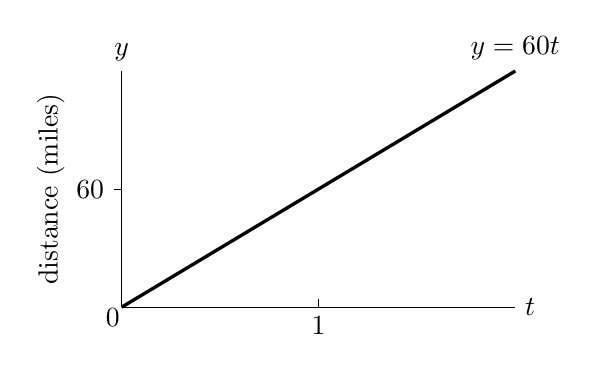
\begin{tikzpicture}[y=3cm,x=5cm]
    \draw (0,0) node[below left=-1mm] {0} -- (0,1) node[above] {$y$} node[rotate=90,pos=0.5,shift={(0,9mm)}] {distance (miles)};
    \draw (0,0.5) -- ++(-1mm,0) node[left] {60};
    \draw (0,0) -- (1,0) node[right] {$t$};
    \draw (0.5,1mm) -- ++(0,-1mm) node[below] {1};
    \draw[very thick] (0,0) -- (1,1) node[above] {$y = 60t$};
\end{tikzpicture}

How far does it travel in \underline{half an hour}?

\begin{tikzpicture}[y=3cm,x=5cm]
    \draw (0,0) node[below left=-1mm] {0} -- (0,1) node[rotate=90,pos=0.5,shift={(0,9mm)}] {speed (miles/hour)};
    \draw (0,0.5) -- ++(-1mm,0) node[left] {60};
    \draw (0,0) -- (1,0) node[right] {$t$} node[below=5mm,pos=0.5] {time (hours)};
    \draw (0.5,1mm) -- ++(0,-1mm) node[below] {1};
    \draw[very thick] (0,0.5) -- (1,0.5);
    \draw (0.25,1mm) -- ++(0,-1mm) node[below] {$\frac{1}{2}$};
    \ifprintanswers
        \begin{pgfonlayer}{background}
            \fill[red!20] (0,0) rectangle (0.25,0.5);
            \draw[line width=0.4mm,{Triangle}-] (0.13,0.3) -- ++(0,0.3) node[above,shift={(9mm,0)}] {Area = 30 miles};
        \end{pgfonlayer}
    \fi
\end{tikzpicture}


\question
A car travels at a speed of 60 miles per hour. 

%...Figures adopted from Strogatz Infinite Powers (p. 170-71)
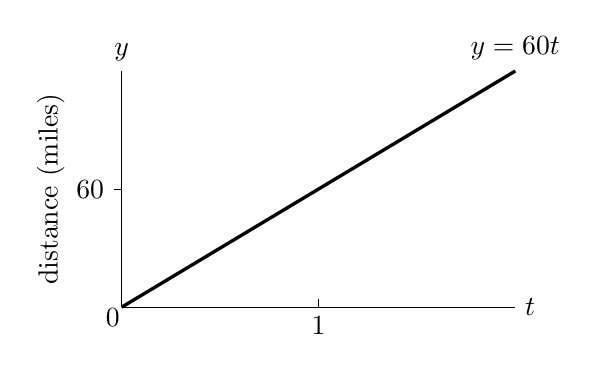
\begin{tikzpicture}[y=3cm,x=5cm]
    \draw (0,0) node[below left=-1mm] {0} -- (0,1) node[above] {$y$} node[rotate=90,pos=0.5,shift={(0,9mm)}] {distance (miles)};
    \draw (0,0.5) -- ++(-1mm,0) node[left] {60};
    \draw (0,0) -- (1,0) node[right] {$t$};
    \draw (0.5,1mm) -- ++(0,-1mm) node[below] {1};
    \draw[very thick] (0,0) -- (1,1) node[above] {$y = 60t$};
\end{tikzpicture}

How far does it travel in \underline{one hour}?

\begin{tikzpicture}[y=3cm,x=5cm]
    \draw (0,0) node[below left=-1mm] {0} -- (0,1) node[rotate=90,pos=0.5,shift={(0,9mm)}] {speed (miles/hour)};
    \draw (0,0.5) -- ++(-1mm,0) node[left] {60};
    \draw (0,0) -- (1,0) node[right] {$t$} node[below=5mm,pos=0.5] {time (hours)};
    \draw (0.5,1mm) -- ++(0,-1mm) node[below] {1};
    \draw[very thick] (0,0.5) -- (1,0.5);
    \draw (0.25,1mm) -- ++(0,-1mm) node[below] {$\frac{1}{2}$};
    \ifprintanswers
        \begin{pgfonlayer}{background}
            \fill[red!20] (0,0) rectangle (0.5,0.5);
            \draw[line width=0.4mm,{Triangle}-] (0.25,0.3) -- ++(0,0.3) node[above,shift={(9mm,0)}] {Area = 60 miles};
        \end{pgfonlayer}
    \fi
\end{tikzpicture}

\vfill\null
\columnbreak

\question
A car travels at a speed of 60 miles per hour. 

%...Figures adopted from Strogatz Infinite Powers (p. 170-71)
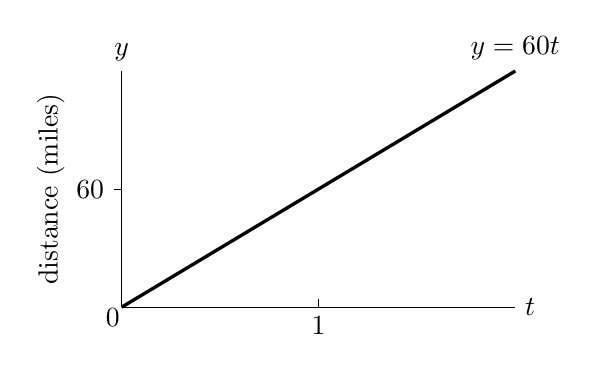
\begin{tikzpicture}[y=3cm,x=5cm]
    \draw (0,0) node[below left=-1mm] {0} -- (0,1) node[above] {$y$} node[rotate=90,pos=0.5,shift={(0,9mm)}] {distance (miles)};
    \draw (0,0.5) -- ++(-1mm,0) node[left] {60};
    \draw (0,0) -- (1,0) node[right] {$t$};
    \draw (0.5,1mm) -- ++(0,-1mm) node[below] {1};
    \draw[very thick] (0,0) -- (1,1) node[above] {$y = 60t$};
\end{tikzpicture}

How far does it travel in \underline{an hour and a half}?

\begin{tikzpicture}[y=3cm,x=5cm]
    \draw (0,0) node[below left=-1mm] {0} -- (0,1) node[rotate=90,pos=0.5,shift={(0,9mm)}] {speed (miles/hour)};
    \draw (0,0.5) -- ++(-1mm,0) node[left] {60};
    \draw (0,0) -- (1,0) node[right] {$t$} node[below=5mm,pos=0.5] {time (hours)};
    \draw (0.5,1mm) -- ++(0,-1mm) node[below] {1};
    \draw[very thick] (0,0.5) -- (1,0.5);
    \draw (0.25,1mm) -- ++(0,-1mm) node[below] {$\frac{1}{2}$};
    \draw (0.75,1mm) -- ++(0,-1mm) node[below] {1.5};
    \ifprintanswers
        \begin{pgfonlayer}{background}
            \fill[red!20] (0,0) rectangle (0.75,0.5);
            \draw[line width=0.4mm,{Triangle}-] (0.38,0.3) -- ++(0,0.3) node[above,shift={(9mm,0)}] {Area = 90 miles};
        \end{pgfonlayer}
    \fi
\end{tikzpicture}

\question
Consider the distance and speed graphs below. 

%...Figures adopted from Strogatz Infinite Powers (p. 170-71)
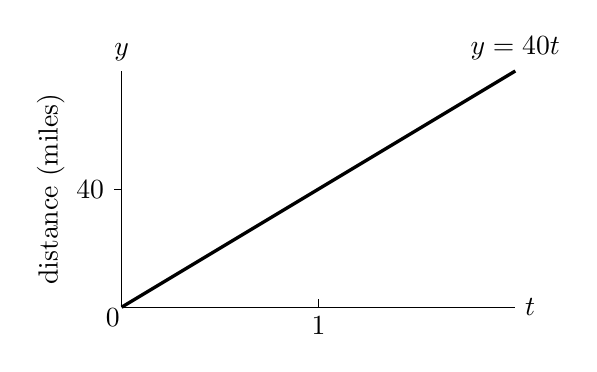
\begin{tikzpicture}[y=3cm,x=5cm]
    \draw (0,0) node[below left=-1mm] {0} -- (0,1) node[above] {$y$} node[rotate=90,pos=0.5,shift={(0,9mm)}] {distance (miles)};
    \draw (0,0.5) -- ++(-1mm,0) node[left] {40};
    \draw (0,0) -- (1,0) node[right] {$t$};
    \draw (0.5,1mm) -- ++(0,-1mm) node[below] {1};
    \draw[very thick] (0,0) -- (1,1) node[above] {$y = 40t$};
\end{tikzpicture}

How far does the object travel in \underline{half an hour}?

\begin{tikzpicture}[y=3cm,x=5cm]
    \draw (0,0) node[below left=-1mm] {0} -- (0,1) node[rotate=90,pos=0.5,shift={(0,9mm)}] {speed (miles/hour)};
    \draw (0,0.5) -- ++(-1mm,0) node[left] {40};
    \draw (0,0) -- (1,0) node[right] {$t$} node[below=5mm,pos=0.5] {time (hours)};
    \draw (0.5,1mm) -- ++(0,-1mm) node[below] {1};
    \draw[very thick] (0,0.5) -- (1,0.5);
    \draw (0.25,1mm) -- ++(0,-1mm) node[below] {$\frac{1}{2}$};
    \draw (0.75,1mm) -- ++(0,-1mm) node[below] {1.5};
    \ifprintanswers
        \begin{pgfonlayer}{background}
            \fill[red!20] (0,0) rectangle (0.25,0.5);
            \draw[line width=0.4mm,{Triangle}-] (0.13,0.3) -- ++(0,0.3) node[above,shift={(9mm,0)}] {Area = 20 miles};
        \end{pgfonlayer}
    \fi
\end{tikzpicture}

\clearpage

\question
How far does the object below travel in \underline{an hour and a half}?

\begin{tikzpicture}[y=3cm,x=5cm]
    \draw (0,0) node[below left=-1mm] {0} -- (0,1) node[rotate=90,pos=0.5,shift={(0,9mm)}] {speed (miles/hour)};
    \draw (0,0.5) -- ++(-1mm,0) node[left] {20};
    \draw (0,0) -- (1,0) node[right] {$t$} node[below=5mm,pos=0.5] {time (hours)};
    \draw (0.5,1mm) -- ++(0,-1mm) node[below] {1};
    \draw[very thick] (0,0.5) -- (1,0.5);
    \draw (0.25,1mm) -- ++(0,-1mm) node[below] {$\frac{1}{2}$};
    \draw (0.75,1mm) -- ++(0,-1mm) node[below] {1.5};
    \ifprintanswers
        \begin{pgfonlayer}{background}
            \fill[red!20] (0,0) rectangle (0.75,0.5);
            \draw[line width=0.4mm,{Triangle}-] (0.38,0.3) -- ++(0,0.3) node[above,shift={(9mm,0)}] {Area = 30 miles};
        \end{pgfonlayer}
    \fi
\end{tikzpicture}

\question
How far does the object travel in \underline{half an hour}?

\begin{tikzpicture}[y=3cm,x=5cm]
    \draw (0,0) node[below left=-1mm] {0} -- (0,1) node[rotate=90,pos=0.5,shift={(0,9mm)}] {speed (miles/hour)};
    \draw (0,0.5) -- ++(-1mm,0) node[left] {50};
    \draw (0,0) -- (1,0) node[right] {$t$} node[below=5mm,pos=0.5] {time (hours)};
    \draw (0.5,1mm) -- ++(0,-1mm) node[below] {1};
    \draw[very thick] (0,0.5) -- (1,0.5);
    \draw (0.25,1mm) -- ++(0,-1mm) node[below] {$\frac{1}{2}$};
    \draw (0.75,1mm) -- ++(0,-1mm) node[below] {1.5};
    \ifprintanswers
        \begin{pgfonlayer}{background}
            \fill[red!20] (0,0) rectangle (0.25,0.5);
            \draw[line width=0.4mm,{Triangle}-] (0.13,0.3) -- ++(0,0.3) node[above,shift={(9mm,0)}] {Area = 25 miles};
        \end{pgfonlayer}
    \fi
\end{tikzpicture}


\question
At \SI{50}{mi/h}, what distance does the object move in 1.5 hours?

\begin{tikzpicture}[y=3cm,x=5cm]
    \draw (0,0) node[below left=-1mm] {0} -- (0,1) node[rotate=90,pos=0.5,shift={(0,9mm)}] {speed (miles/hour)};
    \draw (0,0.5) -- ++(-1mm,0) node[left] {50};
    \draw (0,0) -- (1,0) node[right] {$t$} node[below=5mm,pos=0.5] {time (hours)};
    \draw (0.5,1mm) -- ++(0,-1mm) node[below] {1};
    \draw[very thick] (0,0.5) -- (1,0.5);
    \draw (0.25,1mm) -- ++(0,-1mm) node[below] {$\frac{1}{2}$};
    \draw (0.75,1mm) -- ++(0,-1mm) node[below] {1.5};
    \ifprintanswers
        \begin{pgfonlayer}{background}
            \fill[red!20] (0,0) rectangle (0.75,0.5);
            \draw[line width=0.4mm,{Triangle}-] (0.38,0.3) -- ++(0,0.3) node[above,shift={(9mm,0)}] {Area = 75 miles};
        \end{pgfonlayer}
    \fi
\end{tikzpicture}

\question
How far does the object travel in one hour?

\begin{tikzpicture}[y=3cm,x=5cm]
    \draw (0,0) node[below left=-1mm] {0} -- (0,1) node[rotate=90,pos=0.5,shift={(0,9mm)}] {speed (miles/hour)};
    \draw (0,0.5) -- ++(-1mm,0) node[left] {45};
    \draw (0,0) -- (1,0) node[right] {$t$} node[below=5mm,pos=0.5] {time (hours)};
    \draw (0.5,1mm) -- ++(0,-1mm) node[below] {1};
    \draw[very thick] (0,0.5) -- (1,0.5);
    \draw (0.25,1mm) -- ++(0,-1mm) node[below] {$\frac{1}{2}$};
    \draw (0.75,1mm) -- ++(0,-1mm) node[below] {1.5};
    \ifprintanswers
        \begin{pgfonlayer}{background}
            \fill[red!20] (0,0) rectangle (0.5,0.5);
            \draw[line width=0.4mm,{Triangle}-] (0.25,0.3) -- ++(0,0.3) node[above,shift={(9mm,0)}] {Area = 45 miles};
        \end{pgfonlayer}
    \fi
\end{tikzpicture}

\vfill\null
\columnbreak

\question
Sketch the area accumulated under a speed line for an object moving at 10 miles per hour, for an hour and a half.

\ifprintanswers
\begin{tikzpicture}[y=3cm,x=5cm]
    \draw (0,0) node[below left=-1mm] {0} -- (0,1) node[rotate=90,pos=0.5,shift={(0,9mm)}] {speed (miles/hour)};
    \draw (0,0.5) -- ++(-1mm,0) node[left] {10};
    \draw (0,0) -- (1,0) node[right] {$t$} node[below=5mm,pos=0.5] {time (hours)};
    \draw (0.5,1mm) -- ++(0,-1mm) node[below] {1};
    \draw[very thick] (0,0.5) -- (1,0.5);
    \draw (0.25,1mm) -- ++(0,-1mm) node[below] {$\frac{1}{2}$};
    \draw (0.75,1mm) -- ++(0,-1mm) node[below] {1.5};
    \begin{pgfonlayer}{background}
        \fill[red!20] (0,0) rectangle (0.75,0.5);
        \draw[line width=0.4mm,{Triangle}-] (0.38,0.3) -- ++(0,0.3) node[above,shift={(9mm,0)}] {Area = 15 miles};
    \end{pgfonlayer}
\end{tikzpicture}
\fi

\question
Sketch the area accumulated under a speed line for an object moving at 24 miles per hour, for half an hour.

\ifprintanswers
\begin{tikzpicture}[y=3cm,x=5cm]
    \draw (0,0) node[below left=-1mm] {0} -- (0,1) node[rotate=90,pos=0.5,shift={(0,9mm)}] {speed (miles/hour)};
    \draw (0,0.5) -- ++(-1mm,0) node[left] {24};
    \draw (0,0) -- (1,0) node[right] {$t$} node[below=5mm,pos=0.5] {time (hours)};
    \draw (0.5,1mm) -- ++(0,-1mm) node[below] {1};
    \draw[very thick] (0,0.5) -- (1,0.5);
    \draw (0.25,1mm) -- ++(0,-1mm) node[below] {$\frac{1}{2}$};
    \draw (0.75,1mm) -- ++(0,-1mm) node[below] {1.5};
    \begin{pgfonlayer}{background}
        \fill[red!20] (0,0) rectangle (0.25,0.5);
        \draw[line width=0.4mm,{Triangle}-] (0.13,0.3) -- ++(0,0.3) node[above,shift={(9mm,0)}] {Area = 12 miles};
    \end{pgfonlayer}
\end{tikzpicture}
\fi

\end{multicols}
\end{questions}

\clearpage

\subsection*{LG 7 Practice}

\begin{questions}

\question \label{RpoqN}
The figure below represents the path traveled by a particle in one dimension. (a) Calculate the total distance traveled. (b) Find the displacement.

\positionfigureIII{2}{10}{2}{10}

\begin{solution}
\begin{equation*}
    d = \SI{8}{m} + \SI{8}{m} + \SI{8}{m} = \boxed{\SI{24}{m}}
\end{equation*}

\begin{equation*}
    \Delta x = \SI{10}{m} - \SI{2}{m} = \boxed{\SI{8}{m}}
\end{equation*}
\end{solution}

\question
The figure below represents the path traveled by a particle in one dimension. (a) Calculate the total distance traveled. (b) Find the displacement.

\positionfigureIII{2}{10}{8}{10}

\begin{solution}
\begin{equation*}
    d = \SI{8}{m} + \SI{2}{m} + \SI{2}{m} = \boxed{\SI{12}{m}}
\end{equation*}

\begin{equation*}
    \Delta x = \SI{10}{m} - \SI{2}{m} = \boxed{\SI{8}{m}}
\end{equation*}
\end{solution}


\question
The figure below represents the path traveled by a particle in one dimension. (a) Calculate the total distance traveled. (b) Find the displacement.

\positionfigureIII{0}{10}{5}{12}

\begin{solution}
\begin{equation*}
    d = \SI{10}{m} + \SI{5}{m} + \SI{7}{m} = \boxed{\SI{22}{m}}
\end{equation*}

\begin{equation*}
    \Delta x = \SI{12}{m} - \SI{0}{m} = \boxed{\SI{12}{m}}
\end{equation*}
\end{solution}

\question
The figure below represents the path traveled by a particle in one dimension. (a) Calculate the total distance traveled. (b) Find the displacement.

\positionfigureIII{11}{8}{10}{5}

\begin{solution}
\begin{equation*}
    d = \SI{3}{m} + \SI{2}{m} + \SI{5}{m} = \boxed{\SI{10}{m}}
\end{equation*}

\begin{equation*}
    \Delta x = \SI{5}{m} - \SI{11}{m} = \boxed{\SI{-6}{m}}
\end{equation*}
\end{solution}

\question
The figure below represents the path traveled by a particle in one dimension. (a) Calculate the total distance traveled. (b) Find the displacement.

\positionfigureIII{4}{10}{0}{4}

\begin{solution}
\begin{equation*}
    d = \SI{6}{m} + \SI{10}{m} + \SI{4}{m} = \boxed{\SI{20}{m}}
\end{equation*}

\begin{equation*}
    \Delta x = \SI{4}{m} - \SI{4}{m} = \boxed{0}
\end{equation*}
\end{solution}

\end{questions}

\ifprintanswers \clearpage \fi



\subsection*{LG 8 Practice}

\begin{questions}
\question 
A particle moves point A to point B in 10 seconds. Find the average speed and the average velocity.

\positionfigureIV{-35}{20}

\begin{solution}
\begin{equation*}
    \text{speed} = \frac{\text{distance}}{\text{time}} = \frac{\SI{55}{m}}{\SI{10}{s}} = \boxed{\SI{5.5}{m/s}}
\end{equation*}

\begin{equation*}
    \bar{v} = \frac{\Delta x}{\Delta t} = \frac{\SI{55}{m}}{\SI{10}{s}} = \boxed{\SI{5.5}{m/s}}
\end{equation*}
\end{solution}

\question 
A particle moves point A to point B in 10 seconds. Find the average speed and the average velocity.

\positionfigureIV{45}{-15}

\begin{solution}
\begin{equation*}
    \text{speed} = \frac{\text{distance}}{\text{time}} = \frac{\SI{60}{m}}{\SI{10}{s}} = \boxed{\SI{6}{m/s}}
\end{equation*}

\begin{equation*}
    \bar{v} = \frac{\Delta x}{\Delta t} = \frac{\SI{-60}{m}}{\SI{10}{s}} = \boxed{\SI{-6}{m/s}}
\end{equation*}
\end{solution}

\question 
A particle moves point A to point B in 50 seconds. Find the average speed and the average velocity.

\positionfigureIV{0}{-25}

\begin{solution}
\begin{equation*}
    \text{speed} = \frac{\text{distance}}{\text{time}} = \frac{\SI{25}{m}}{\SI{50}{s}} = \boxed{\SI{0.5}{m/s}}
\end{equation*}

\begin{equation*}
    \bar{v} = \frac{\Delta x}{\Delta t} = \frac{\SI{-25}{m}}{\SI{50}{s}} = \boxed{\SI{-0.5}{m/s}}
\end{equation*}
\end{solution}

\question 
A particle moves point A to point B in 25 seconds. Find the average speed and the average velocity.

\positionfigureIV{35}{-40}

\begin{solution}
\begin{equation*}
    \text{speed} = \frac{\text{distance}}{\text{time}} = \frac{\SI{75}{m}}{\SI{25}{s}} = \boxed{\SI{3.0}{m/s}}
\end{equation*}

\begin{equation*}
    \bar{v} = \frac{\Delta x}{\Delta t} = \frac{\SI{-75}{m}}{\SI{25}{s}} = \boxed{\SI{-3.0}{m/s}}
\end{equation*}
\end{solution}

\question 
A particle moves point A to point B in 4 seconds. Find the average speed and the average velocity.

\positionfigureIV{15}{-45}

\begin{solution}
\begin{equation*}
    \text{speed} = \frac{\text{distance}}{\text{time}} = \frac{\SI{60}{m}}{\SI{4}{s}} = \boxed{\SI{15}{m/s}}
\end{equation*}

\begin{equation*}
    \bar{v} = \frac{\Delta x}{\Delta t} = \frac{\SI{-60}{m}}{\SI{4}{s}} = \boxed{\SI{-15}{m/s}}
\end{equation*}
\end{solution}


\end{questions}

\clearpage

\subsection*{LG 9 Practice}

\textbf{Questions \ref{6NK1K}--\ref{dr2on}.} Below, will you will draw motion maps for a particle. In each figure, the side of each grid square represents 1 meter of distance.

\begin{questions}

\question \label{6NK1K}
A particle travels at a constant  speed of \SI{2}{m/s} in the negative direction. Draw a motion map for the particle. Label the initial and final positions, and direction of velocity.

\begin{center}
    \positionfigureVI{2}
\end{center}

\question
A particle travels at a constant  speed of \SI{6}{m/s} in the negative direction. Draw a motion map for the particle. Label the initial and final positions, and direction of velocity.

\begin{center}
    \positionfigureVI{6}
\end{center}

\question
A particle travels at a constant  speed of \SI{3}{m/s} in the negative direction. Draw a motion map for the particle. Label the initial and final positions, and direction of velocity.

\begin{center}
    \positionfigureVI{3}
\end{center}

\question
A particle travels at a constant  speed of \SI{4}{m/s} in the negative direction. Draw a motion map for the particle. Label the initial and final positions, and direction of velocity.

\begin{center}
    \positionfigureVI{4}
\end{center}

\question 
A particle travels at a constant  speed of \SI{8}{m/s} in the negative direction. Draw a motion map for the particle. Label the initial and final positions, and direction of velocity.

\begin{center}
    \positionfigureVI{8}
\end{center}

\question \label{dr2on}
A particle travels at a constant  speed of \SI{1}{m/s} in the negative direction. Draw a motion map for the particle. Label the initial and final positions, and direction of velocity.

\begin{center}
    \positionfigureVI{1}
\end{center}
\end{questions}

\clearpage

\subsection*{Review LG 1--8}

\begin{questions}
\question
The following table shows 8 physical quantities that we've covered so far. Search your memory to fill in the missing information in the table. The completed first row is shown as an example.
\vspace{-2em}

\begin{EnvUplevel}
\def\arraystretch{1.5}
\begin{center}
\begin{tabular}{|w{c}{1cm}|w{c}{4cm}||w{c}{5cm}|w{c}{1.5cm}||w{c}{2cm}|}
    \hline
    \thead{\bfseries Symbol} & \thead{\bfseries Quantity} & \thead{\bfseries SI Unit} & \thead{\bfseries Unit\\ \bfseries Symbol} & \thead{\bfseries Example}\\ \hline
    $x$ & position & meters & m & $x = \SI{5}{m}$ \\ \hline 
    \ans{D} & distance & \ans{meters} & m & \ans{$\mathrm{D} = \SI{10}{m}$} \\ \hline 
    S & speed & \ans{meters per second} & \ans{m/s} & \ans{$\mathrm{S} = \SI{7}{m/s}$} \\ \hline 
    T & \ans{time} & \ans{seconds} & s & \ans{$\mathrm{T} = \SI{45}{s}$} \\ \hline 
    $x_f$ & \ans{final position} & meters & m & \ans{$x_f = -\SI{8}{m}$} \\ \hline 
    \ans{$x_i$} & initial position & \ans{meters} & \ans{m} & \ans{$x_i = +\SI{5}{m}$} \\ \hline 
    \ans{$\Delta x$} & displacement & meters & \ans{m} & \ans{$\Delta x = -\SI{3}{m}$} \\ \hline 
    $v$ & \ans{velocity} & \ans{meters per second} & m/s & \ans{$v = -\SI{4}{m/s}$} \\ \hline 
\end{tabular}
\end{center}
\end{EnvUplevel}

\question
The figure below is a one-dimensional position axis. 

\begin{parts}
\part Choose any initial position, then draw a path along which an object changes direction twice. Label the initial and final positions using the appropriate variables.

\begin{center}
\begin{tikzpicture}[y=3mm,x=8mm]
    \draw[black!10,xstep=1,ystep=2] (0,0) grid (12,4);
    \foreach \x in {0,1,...,12} {
        \draw[ultra thin] (\x,-1mm) -- (\x,1mm) node[below=3mm] {$\x$};
    }
    \draw[->] (0,0) -- (12,0) node[right=1mm] {$x$ (m)};
    \ifprintanswers
        \node[red] at (6,2) {\bfseries Answers will vary.};
    \fi
\end{tikzpicture}
\end{center}

\part Calculate the total distance traveled by your object.

\begin{solutionorbox}[2.5cm]
    Answers will vary.
\end{solutionorbox}

\part Calculate the object's displacement, showing all your working, including the formula used.

\begin{solutionorbox}[1.5cm]
    Answers will vary.
\end{solutionorbox}

\part Calculate your object's \underline{speed} if the travel time was 10 seconds. Then, find it's \underline{average velocity} for the same time interval.

\begin{solutionorbox}[3.5cm]
    Answers will vary.
\end{solutionorbox}
\end{parts}

\ifprintanswers \else \clearpage \fi

\question
In the space below, draw the DST triangle. Then, use it to write down 3 equations for distance, speed, and time. 

\begin{solutionorbox}[2.8cm]

\centering
\begin{minipage}{4cm}
\centering

\DSTtriangle[shade=D]

\begin{equation*}
    \mathrm{distance = speed \times time}
\end{equation*}
\end{minipage}%
\hspace{5mm}
\begin{minipage}{4cm}
\centering

\DSTtriangle[shade=S]

\begin{equation*}
    \mathrm{speed = \frac{distance}{time}}
\end{equation*}
\end{minipage}%
\hspace{5mm}
\begin{minipage}{4cm}
\centering

\DSTtriangle[shade=T]

\begin{equation*}
    \mathrm{time = \frac{distance}{speed}}
\end{equation*}
\end{minipage}%

\end{solutionorbox}

\question
Label the points below as $\left(x_1,y_1\right)$ and $\left(x_2,y_2\right)$. Then, find the slope of the line. Show all your work. 

\begin{EnvUplevel}
\centering

\begin{minipage}[t]{8cm}
\vspace{0pt}%
\centering
\begin{tikzpicture}
    \begin{axis}[height=7.6cm,width=8.5cm,
        axis lines=center,
        ylabel={$y$},
        xlabel={$x$},
        ymin=-10,ymax=10,
        xmin=-10,xmax=10,
        ytick={-10,-8,...,10},
        xtick={-10,-8,...,10},
        grid=both, 
        minor y tick num=1,
        minor x tick num=1,
    ]
        \addplot[thick,domain=-10:10] {5/3*x -8};
        \fill (0,-8) circle (3pt);
        \fill (6,2) circle (3pt);
        \ifprintanswers
        \node[red,align=center,right=2mm] at (0,-8) {$(x_1,y_1)$\\[1ex]$(0,-8)$};
        \node[red,align=center,above left=-2mm] at (6,2) {$(x_2,y_2)$\\[1ex]$(6,2)$};
        \fi
    \end{axis}
\end{tikzpicture}
\end{minipage}%
\fbox{
\begin{minipage}[t]{7.5cm}
\vspace{0pt}%
\centering
\textcolor{white}{\rule{7.5cm}{0.4pt}}
{\ifprintanswers \color{red} \else \color{white} \fi
\begin{align*}
    \text{slope} = m &= \mathrm{\frac{rise}{run}} \\[1ex]
    &= \frac{y_2 - y_1}{x_2 - x_1} \\[1ex]
    &= \frac{2 - (-8)}{6 - 0} \\[1ex]
    &= \frac{10}{6} \\[1ex]
    &= \boxed{\frac{5}{3}} \approx 1.667
\end{align*}
}
\vspace{7mm}
\end{minipage}}
\end{EnvUplevel}

\question
If you’re given a distance vs.\,time graph for an object traveling at a constant speed, how can you use the graph to find the object’s speed?

\ifprintanswers
\textcolor{red}{The speed of the object on a distance vs.\,time graph is the slope of the line. Therefore, to find the speed you need to calculate the slope.}
\else
\fillwithlines{14mm}
\fi

\question
Explain which physical quantity is represented by the shaded region in the graph below.

\begin{center}
\begin{minipage}[t]{6cm}
\vspace{0pt}%
\centering
\begin{tikzpicture}
    \begin{axis}[height=4cm,width=6cm,
        axis lines=left,
        ylabel = {Speed (m/s)},
        xlabel = {Time (s)},
        ymin=0, ymax=4,
        xmin=0, xmax=6,
        ytick={0,1,...,4},
        xtick={0,1,...,6},
        grid=both,
        ]
        \addplot[very thick,domain=0:6] {3};
        \begin{pgfonlayer}{background}
            \fill[black!12] (0,0) rectangle (4,3);
        \end{pgfonlayer}
    \end{axis}
\end{tikzpicture}
\end{minipage}%
\hspace{5mm}
\fbox{
\begin{minipage}[t]{8cm}
\vspace{0pt}%
{\ifprintanswers \color{red} \else \color{white} \fi

\noindent The region is a rectangle with a ``width'' of speed and a ``length'' of time. Since 
\vspace{-1ex}

\begin{align*}
    \mathrm{area} &= \mathrm{length \times width} \\
    &\text{and} \\
    \mathrm{distance} &= \mathrm{speed \times time} \quad ,
\end{align*}

the area of the rectangle is equivalent to the distance traveled by the object.}
\end{minipage}}
\end{center}

\question
(a) Choose a constant speed less than 10 m/s: \fillin[{\scriptsize answers will vary}][2.5cm]. (b) Draw a motion map for a particle moving at that speed, in the figure below. Label times and initial and final positions in the figure.
\vspace{1em}

\begin{tikzpicture}[y=6mm,x=6mm]
    \draw[black!20,step=1] (0,0) grid (24,2);  
    \draw[|-|] (0,-0.3) -- ++(2,0) node[below,pos=0.5] {\small 1 meter};
    \ifprintanswers
    \node[red,fill=black!10] at (12,1) {answers will vary};
    \fi
\end{tikzpicture}
\clearpage

\end{questions}

\clearpage

\subsection*{Quiz on position, displacement, speed, and velocity}

\begin{questions}

\question
A particle travels from point A to point B.

\positionfigureII{3}{-4}

The distance traveled is given by\ldots

\begin{randomizechoices}
    \correctchoice $\displaystyle \big|A - B\big|$
    \choice $\displaystyle \big|A + B\big|$
    \choice $\displaystyle \big|A \times B\big|$
    \choice $\displaystyle \big|A \div B\big|$
\end{randomizechoices}



\question
Isaac jogs across a 28 meter patch of grass at a rate of 4 meters per second. How much time does it take Isaac to cross the patch?

\begin{randomizechoices}
    \correctchoice \SI{7}{s}
    \choice \SI{112}{s}
    \choice \SI{0.14}{s}
    \choice \SI{8}{s}
\end{randomizechoices}

\question Find the slope of the line.

\xygraphI{3}{-4}{(0,-4)(2,2)}

\begin{randomizechoices}
    \correctchoice $3$
    \choice $\frac{1}{3}$
    \choice $-3$
    \choice $-\frac{1}{3}$
\end{randomizechoices}

\question
What is the speed of the car shown below?

\distancegraphI{25}

\begin{randomizechoices}
    \correctchoice \SI{25}{mi/h}
    \choice \SI{100}{mi/h}
    \choice \SI{50}{mi/h}
    \choice \SI{12}{mi/h}
\end{randomizechoices}

\question
What is the formula for finding the area of the rectangle?
\vspace{1em}

\rectangleI{5}{3}{7}
\vspace{1em}

\begin{randomizechoices}
    \correctchoice $\mathrm{length \times width}$
    \choice $\mathrm{length + width}$
    \choice $\mathrm{length \div width}$
    \choice $\mathrm{length - width}$
\end{randomizechoices}

\question
What physical quantity does the shaded area in the figure below represent?

\begin{center}
\begin{tikzpicture}[y=3cm,x=5cm]
    \draw (0,0) node[below left=-1mm] {0} -- (0,1) node[rotate=90,pos=0.5,shift={(0,9mm)}] {speed (miles/hour)};
    \draw (0,0.5) -- ++(-1mm,0) node[left] {60};
    \draw (0,0) -- (1,0) node[right] {$t$} node[below=5mm,pos=0.5] {time (hours)};
    \draw (0.5,1mm) -- ++(0,-1mm) node[below] {1};
    \draw[very thick] (0,0.5) -- (1,0.5);
    \draw (0.25,1mm) -- ++(0,-1mm) node[below] {$\frac{1}{2}$};
    \draw (0.75,1mm) -- ++(0,-1mm) node[below] {1.5};
    \begin{pgfonlayer}{background}
        \fill[black!15] (0,0) rectangle (0.75,0.5);
        \draw[line width=0.4mm,{Triangle}-] (0.38,0.3) -- ++(0,0.3);
    \end{pgfonlayer}
\end{tikzpicture}
\end{center}

\begin{randomizechoices}
    \correctchoice the distance traveled by the object
    \choice the speed of the object
    \choice the slope of object's motion
    \choice the amount of time traveled by the object
\end{randomizechoices}

\question
A particle moves in one dimension, turning around twice, as shown in the figure. Calculate the particle's displacement.

\positionfigureIII{8}{2}{7}{5}


\begin{randomizechoices}
    \correctchoice \SI{-3}{m}
    \choice \SI{3}{m}
    \choice \SI{-13}{m}
    \choice \SI{13}{m}
\end{randomizechoices}


\question
A particle travels from point A to point B in 2 seconds. What is the average velocity?

\positionfigureII{5}{-3}

\begin{randomizechoices}
    \correctchoice $-\SI{4}{m/s}$
    \choice $+\SI{4}{m/s}$
    \choice $-\SI{8}{m/s}$
    \choice $+\SI{8}{m/s}$
\end{randomizechoices}

\question
The following motion map shows an object moving at constant speed. $\Delta x_1$ and $\Delta x_5$ represent the object's displacements in the 1st and 5th time intervals, respectively.

\begin{center}
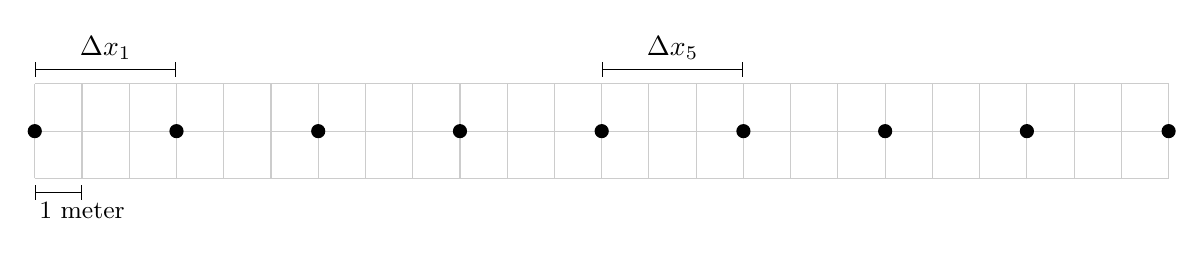
\begin{tikzpicture}[y=6mm,x=6mm]
    \draw[black!20,step=1] (0,0) grid (24,2);  
    \draw[|-|] (0,-0.3) -- ++(1,0) node[below] {\small 1 meter};
    \foreach \x in {0,3,...,24}{
        \fill (\x,1) circle (0.9mm);
    }
    \draw[|-|] (0,2.3) -- ++(3,0) node[above,pos=0.5] {$\Delta x_1$};
    \draw[|-|] (12,2.3) -- ++(3,0) node[above,pos=0.5] {$\Delta x_5$};
\end{tikzpicture}
\end{center}

How do sizes of the two displacements compare?

\begin{randomizechoices}[keeplast]
    \correctchoice The two displacements are equal $\left(\Delta x_1 = \Delta x_5\right)$.
    \choice The displacement in the 1st time interval is greater $\left(\Delta x_1 > \Delta x_5\right)$.
    \choice The displacement in the 5th time interval is greater $\left(\Delta x_1 < \Delta x_5\right)$.
    \choice There's no way to compare displacements without knowing the object's speed.
\end{randomizechoices}

\question
What do $x$ and $\Delta x$ represent in physics?

\begin{randomizechoices}
    \correctchoice $x$ is for position, and $\Delta x$ is for displacement (change in position).
    \choice $x$ is for displacement, and $\Delta x$ is for position (change in displacement).
    \choice $x$ is for distance, and $\Delta x$ is for position (change in distance).
    \choice $x$ is for position, and $\Delta x$ is for distance (change in position).
\end{randomizechoices}

\end{questions}

\clearpage

\subsection*{Lab: The Dune Buggy}

\begin{center}
\begin{minipage}{4.5cm}
\noindent \textit{Materials}:
\vspace{-2ex}

\begin{center}
\begin{itemize}[itemsep=0pt,topsep=2pt]
    \item dune buggy
    \item track
    \item tape
    \item metronome (laptop)
\end{itemize}
\end{center}
\end{minipage}%
\begin{minipage}{10.5cm}
\centering
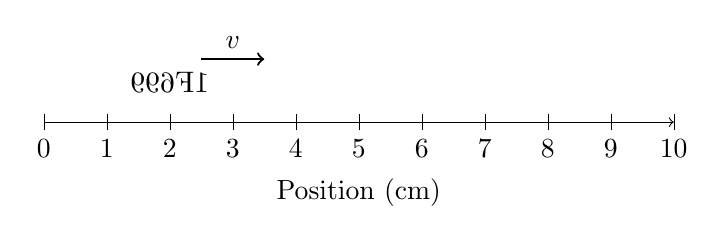
\begin{tikzpicture}[y=8mm,x=8mm]
    \foreach \x in {0,1,...,10} {
        \draw[ultra thin] (\x,-1mm) -- (\x,1mm) node[below=2mm] {$\x$};
    }
    \draw[->] (0,0) -- (10,0) node[below=6mm,pos=0.5] {Position (cm)};
    \node[shift={(0,5mm)}] at (2,0) {\resizebox{1cm}{!}{\reflectbox{\usym{1F699}}}};
    \draw[->,thick] (2.5,1) --++ (1,0) node[above,pos=0.5] {$v$};
\end{tikzpicture} 
\end{minipage}
\end{center}
\vspace{1ex}

{\bfseries \noindent Part I: Constant Positive Velocity}
\vspace{1ex}

\noindent \textit{Procedure:}

\begin{enumerate}[itemsep=0pt,topsep=2pt]
\item Place the dune buggy at the origin $\left(x_i = 0\right)$.
\item Set the Google metronome at 60\,BPM, yielding 1 beat per second.
\item Release the buggy at 0\,cm, exactly on the sound of a beat. Call this ``beat 0.''
\item For each subsequent beat, place a tape strip on the track, at the buggy’s location for that beat.
\item Use a meterstick to measure the displacements between tape strips, recording data in the table below. Then, take the ratio of subsequent displacements to the first displacement (see column 3).

\begin{center}
\def\arraystretch{2}
\begin{tabular}{|w{c}{3cm}|w{l}{5cm}|w{l}{2.5cm}|}
    \hline
    \thead{\bfseries Time Interval} & \thead{\bfseries Interval Displacement (cm)} & \thead{\bfseries Ratio $\Delta x_n/\Delta x_1$} \\ \hline
    Beat 0 to 1 & $\Delta x_1 =$ \ans{.} & $\displaystyle \frac{\Delta x_1}{\Delta x_1} = $ \\[1ex] \hline 
    Beat 1 to 2 & $\Delta x_2 =$ \ans{.} & $\displaystyle \frac{\Delta x_2}{\Delta x_1} = $ \\[1ex] \hline 
    Beat 2 to 3 & $\Delta x_3 =$ \ans{.} & $\displaystyle \frac{\Delta x_3}{\Delta x_1} = $ \\[1ex] \hline 
    Beat 3 to 4 & $\Delta x_4 =$ \ans{.} & $\displaystyle \frac{\Delta x_4}{\Delta x_1} = $ \\[1ex] \hline 
    Beat 4 to 5 & $\Delta x_5 =$ \ans{.} & $\displaystyle \frac{\Delta x_5}{\Delta x_1} = $ \\[1ex] \hline 
    Beat 5 to 6 & $\Delta x_6 =$ \ans{.} & $\displaystyle \frac{\Delta x_6}{\Delta x_1} = $ \\[1ex] \hline 
\end{tabular}
\end{center}

\item Record the positions of the tape strips in the table below, then plot the data on the graph.

\begin{center}
\begin{minipage}{4cm}
\centering
\def\arraystretch{1.8}
\begin{tabular}{|w{c}{1.5cm}|w{c}{1.5cm}|}
    \hline
    \thead{\bfseries Time\\ \bfseries (s)} & \thead{\bfseries Position\\ \bfseries (cm)} \\ \hline
    0 & 0 \\ \hline 
    1 & \ans{.} \\ \hline 
    2 & \ans{.} \\ \hline 
    3 & \ans{.} \\ \hline 
    4 & \ans{.} \\ \hline 
    5 & \ans{.} \\ \hline 
    6 & \ans{.} \\ \hline 
\end{tabular}
\end{minipage}%
\hspace{5mm}
\begin{minipage}{10.5cm}
\centering
\begin{tikzpicture}
    \begin{axis}[height=7cm,width=10cm,
        ylabel={Position (cm)},
        xlabel={Time (s)},
        ymin=0,ymax=120,
        xmin=0,xmax=6,
        ytick={0,20,...,120},
        xtick={0,1,...,6},
        axis lines=left,
        grid=both,
        minor y tick num=1,
        minor x tick num=1
    ]
    \ifprintanswers
    \addplot[red!50!black,domain=0:20] {0.399*x};
    \addplot[mark=*,only marks,red,mark size=2pt] coordinates{(0,0)(2.7,1)(5.3,2)(7.6,3)(10.1,4)(12.6,5)(15.2,6)(17.6,7)(20.2,8)};
    \fi
    \end{axis}
\end{tikzpicture}
\end{minipage}
\end{center}

\clearpage

\item Draw a best-fit line to the points on the graph above.


\item Calculate the slope of the best-fit line, with correct units.
\vspace{-1ex}

\begin{center}
\fbox{
\begin{minipage}{14.5cm}
\vspace{1ex}
{\ifprintanswers \color{red} \else \color{white} \fi

\begin{align*}
    \text{slope} &= \frac{\Delta x}{\Delta x} \\[1ex]
    &= \frac{x_2 - x_1}{t_2 - t_1} \\[1ex]
    &= \boxed{\SI{}{m/s}}
\end{align*}
}
\vspace{1.5cm}
\end{minipage}}
\end{center}
\end{enumerate}


{\bfseries \noindent Part II: Constant Negative Velocity}
\vspace{1ex}

\noindent \textit{Procedure:}

\begin{enumerate}[itemsep=0pt,topsep=2pt]
\item Place the dune buggy at track's end $\left(x_i = \SI{120}{cm}\right)$.
\item Release the buggy at 120\,cm, exactly on the sound of a beat, this time with negative (leftward) velocity.
\item Like before, for each subsequent beat, place a tape strip on the track at the buggy’s location.
\item Record the positions of the tape strips in the table below, then plot the data on the graph.

\begin{center}
\begin{minipage}{4cm}
\centering
\def\arraystretch{1.8}
\begin{tabular}{|w{c}{1.5cm}|w{c}{1.5cm}|}
    \hline
    \thead{\bfseries Time\\ \bfseries (s)} & \thead{\bfseries Position\\ \bfseries (cm)} \\ \hline
    0 & 120 \\ \hline 
    1 & \ans{.} \\ \hline 
    2 & \ans{.} \\ \hline 
    3 & \ans{.} \\ \hline 
    4 & \ans{.} \\ \hline 
    5 & \ans{.} \\ \hline 
    6 & \ans{.} \\ \hline 
\end{tabular}
\end{minipage}%
\hspace{5mm}
\begin{minipage}{10.5cm}
\centering
\begin{tikzpicture}
    \begin{axis}[height=7cm,width=10cm,
        ylabel={Position (cm)},
        xlabel={Time (s)},
        ymin=0,ymax=120,
        xmin=0,xmax=6,
        ytick={0,20,...,120},
        xtick={0,1,...,6},
        % xticklabels=\empty,
        % yticklabels=\empty,
        axis lines=left,
        grid=both,
        minor y tick num=1,
        minor x tick num=1
    ]
    \ifprintanswers
    \addplot[red!50!black,domain=0:20] {0.399*x};
    \addplot[mark=*,only marks,red,mark size=2pt] coordinates{(0,0)(2.7,1)(5.3,2)(7.6,3)(10.1,4)(12.6,5)(15.2,6)(17.6,7)(20.2,8)};
    \fi
    \end{axis}
\end{tikzpicture}
\end{minipage}
\end{center}

\item Draw a best-fit line to the points on the graph.

\item Calculate the slope of the best-fit line, with correct units.
\vspace{-1ex}

\begin{center}
\fbox{
\begin{minipage}{14.5cm}
\vspace{1ex}
{\ifprintanswers \color{red} \else \color{white} \fi

\begin{align*}
    \text{slope} &= \frac{\Delta x}{\Delta x} \\[1ex]
    &= \frac{x_2 - x_1}{t_2 - t_1} \\[1ex]
    &= \boxed{\SI{}{m/s}}
\end{align*}
}
\vspace{1.5cm}
\end{minipage}}
\end{center}
\end{enumerate}

\clearpage

{\noindent \bfseries Analysis}

\begin{questions}

% \question Calculate the slope of the best-fit line, with the correct units. (Answers may vary.)

% \begin{solutionorbox}[6cm]
%     To find slope, choose any two points and compute rise (change in position) over run (change in time). For example, choosing coordinates

%     \begin{equation*}
%         (t_1,x_2) = (\SI{5.3}{s},\SI{2}{m}) \qquad \text{and} \qquad
%         (t_2,x_1) = (\SI{15.2}{s},\SI{6}{m})
%     \end{equation*}
    
%     the slope is

%     \begin{equation*}
%         \text{slope} = \frac{x_2 - x_1}{t_2 - t_1} 
%         = \frac{\SI{6}{m} - \SI{2}{m}}{\SI{15.2}{s} - \SI{5.3}{s}} = \boxed{\SI{0.404}{m/s}}
%     \end{equation*}

%     \bigskip

%     On a calculator, use parentheses like this:

%     \medskip

%     \begin{center}
%         \texttt{(6-2)/(15.2-5.3)}\\
%         \hspace{2.5em} \texttt{.404040404}
%     \end{center}
% \end{solutionorbox}

\question
What physical quantity does the slope represent in each position vs.\,time graph?

\ifprintanswers
{\color{red}
On the position-vs-time graph, the rise is a change in position ($\Delta x$), and the run is a change in time ($\Delta t$). Therefore, slope is

\begin{equation*}
    \text{slope} = \mathrm{\frac{rise}{run}} = \frac{\Delta x}{\Delta t}
\end{equation*}

But $\Delta x$ means displacement, and the ratio $\Delta x/\Delta t$ represents average velocity. Therefore, the slope is the dune buggy's velocity.
}
\else
\fillwithlines{14mm}
\fi

\question
What does the sign ($+$ or $-$) of the slope tell you about the motion of the buggy?

\ifprintanswers 
\else \fillwithlines{14mm}
\fi

\question
In both graphs above, there is a $y$-intercept, a point where the line intersects the vertical (position) axis. What physical quantity does the $y$-intercept represent for the buggy?

\ifprintanswers 
\else \fillwithlines{14mm}
\fi


\question
In each trial, did your dune buggy move at a constant speed? How do you know?

\ifprintanswers 
\else \fillwithlines{14mm}
\fi

\question
How can you determine from your graph if your car is moving faster or slower than another car?

\ifprintanswers 
\else \fillwithlines{14mm}
\fi


\question
In Part I, you calculated the ratio of each displacement to the first interval displacement $\displaystyle \left(\frac{\Delta x_n}{\Delta x_1}\right)$. 

\begin{parts}
\part What ideal value should this ratio equal for every interval?

\ifprintanswers 
\else \fillwithlines{14mm}
\fi

\part What does this tell you about the buggy's velocity over equal time intervals?

\ifprintanswers 
\else \fillwithlines{14mm}
\fi
\end{parts}


\question

\begin{parts}
\part If the buggy's battery began dying halfway through the run, how would the interval displacements ($\Delta x_n$) change?

\ifprintanswers 
\else \fillwithlines{14mm}
\fi

\part What would happen to the slope of your position-vs-time graph? 

\ifprintanswers 
\else \fillwithlines{14mm}
\fi
\end{parts}

\question
Summarize an important idea(s) you learned in doing this lab.

\ifprintanswers 
\else \fillwithlines{14mm}
\fi

\clearpage

% \question Write the linear equation for the dune buggy's position as a function of time.

% \ifprintanswers
% {\color{red}
% \begin{equation*}
%     x = (\SI{0.40}{m/s})\, t
% \end{equation*}
% }
% \else 
% \fillwithlines{7mm}
% \fi

\end{questions}

\clearpage


\subsection*{LG 10 Practice}

\begin{questions}

\question 
Draw the position vector for the person below.

\positionfigureI{3}

\question 
Draw the position vector for the person below.

\positionfigureI{-2}

\question 
Draw the position vector for the person below.

\positionfigureI{-5}

\question 
Draw the position vector for the person below.

\positionfigureI{1}

\question 
Draw the position vector for the person below.

\positionfigureI{4}

\question 
Draw the position vector for the person below.

\positionfigureI{-3}

\question 
Draw the position vector for the person below.

\positionfigureI{5}

\end{questions}

\clearpage

\subsection*{LG 11 Practice}

\textbf{Questions \ref{pPNfs}--\ref{Yi2yY}.} The figure below shows a one-dimensional  position axis, with an object currently at the origin. By convention, motion in the rightward direction is defined as positive $\left(+\right)$.

\begin{center}
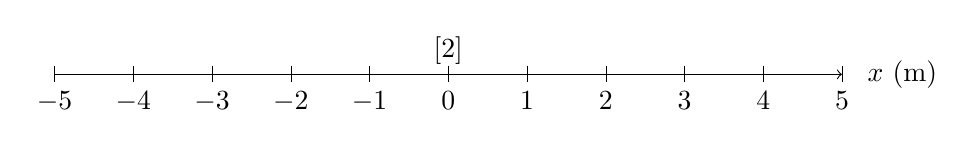
\begin{tikzpicture}[y=1cm,x=1cm]
    \foreach \x in {-5,-4,...,5} {
        \draw[ultra thin] (\x,-1mm) -- (\x,1mm) node[below=2mm] {$\x$};
    }
    \draw[->] (-5,0) -- (5,0) node[right=2mm] {$x$ (m)};
    \node[above] at (0,0) {\Strichmaxerl[2]};
    % \ifprintanswers
    %     \draw[very thick,->,red] (0,0.7) -- ++(#1,0) node[above,pos=0.5] {$\vec{x}$};
    % \fi
\end{tikzpicture}  
\end{center}

\begin{questions}
\question \label{pPNfs}
A particle's position and velocity vectors are:

\begin{equation*}
    \vec{x} = \SI{24}{m}\ , \quad \vec{v} = -\SI{6}{m/s}    
\end{equation*}


Is the particle moving toward or away from the origin?

\ifprintanswers \textcolor{red}{Toward the origin.} \fi

\question %2
A particle's position and velocity vectors are:

\begin{equation*}
    \vec{x} = \SI{4}{m}\ , \quad \vec{v} = \SI{7}{m/s}
\end{equation*}


In which direction is the object moving?

\ifprintanswers \textcolor{red}{To the right.} \fi

\question %5
A particle's position and velocity vectors are:

\begin{equation*}
    \vec{x} = -\SI{56}{m}\ , \quad \vec{v} = +\SI{10}{m/s}
\end{equation*}


Is the particle moving toward or away from the origin?

\ifprintanswers \textcolor{red}{Toward the origin.} \fi


\question %8
A particle's position and velocity vectors are:

\begin{equation*}
    \vec{x} = -\SI{13}{m}\ , \quad \vec{v} = -\SI{35}{m/s}    
\end{equation*}


Is the particle moving toward or away from the origin?

\ifprintanswers \textcolor{red}{Away from the origin}. \fi

\question %1
A particle's position and velocity vectors are:

\begin{equation*}
    \vec{x} = +\SI{2}{m}\ , \quad \vec{v} = -\SI{5}{m/s}
\end{equation*}

In which direction is the object moving?

\ifprintanswers \textcolor{red}{To the left.} \fi

\question %3
A particle's position and velocity vectors are:

\begin{equation*}
    \vec{x} = -\SI{12}{m}\ , \quad \vec{v} = \SI{23}{m/s}
\end{equation*}

In which direction is the object moving?

\ifprintanswers \textcolor{red}{To the right.} \fi


\question %6
A particle's position and velocity vectors are:

\begin{equation*}
    \vec{x} = \SI{12}{m}\ , \quad \vec{v} = \SI{15}{m/s}    
\end{equation*}


Is the particle moving toward or away from the origin?

\ifprintanswers \textcolor{red}{Away from the origin}. \fi


\question \label{Yi2yY}
A particle's position and velocity vectors are:

\begin{equation*}
    \vec{x} = -\SI{15}{m}\ , \quad \vec{v} = -\SI{6}{m/s} 
\end{equation*}


In which direction is the object moving?

\ifprintanswers \textcolor{red}{To the left.} \fi


\end{questions}

\clearpage

\subsection*{LG 12 Practice}

\textbf{Questions \ref{BuZsv}--\ref{unser}.} 
For each problem below, Figure 1 displays 5 vectors. Use the head-to-tail method to graphically add all vectors, showing your work in Figure 2. Then, in the space above Figure 2, draw the resultant vector.

\begin{questions}
\question \label{BuZsv}
\phantom{.}
\vspace{-1em}

\begin{center}
    \positionfigureV{-6}{6}{8}{5}{-9}{13}
\end{center}

% \begin{solution}
% \begin{equation*}
%     \Delta x_\text{\scriptsize net} = \SI{-6}{m} + \SI{6}{m} + \SI{8}{m} + \SI{5}{m} + (\SI{-9}{m}) = \boxed{\SI{4}{m}}
% \end{equation*}
% \end{solution}


\question
\phantom{.}
\vspace{-1em}

\begin{center}
    \positionfigureV{2}{-3}{6}{-1}{-2}{10}
\end{center}

% \begin{solution}
% \begin{equation*}
%     \Delta x_\text{\scriptsize net} = \SI{2}{m} + (\SI{-3}{m}) + \SI{5}{m} + (\SI{-1}{m}) + (\SI{-2}{m}) = \boxed{\SI{1}{m}}
% \end{equation*}
% \end{solution}


\question
\phantom{.}
\vspace{-1em}

\begin{center}
    \positionfigureV{3}{-5}{7}{-2}{2}{10}    
\end{center}

% \begin{solution}
% \begin{equation*}
%     \Delta x_\text{\scriptsize net} = \SI{3}{m} + (\SI{-5}{m}) + \SI{7}{m} + (\SI{-2}{m}) + \SI{1}{m} = \boxed{\SI{4}{m}}
% \end{equation*}
% \end{solution}

\question
\phantom{.}
\vspace{-1em}

\begin{center}
    \positionfigureV{7}{-9}{1}{-3}{2}{10}
\end{center}

% \begin{solution}
% \begin{equation*}
%     \Delta x_\text{\scriptsize net} = \SI{7}{m} + (\SI{-9}{m}) + \SI{1}{m} + (\SI{-3}{m}) + \SI{2}{m} = \boxed{\SI{-2}{m}}
% \end{equation*}
% \end{solution}

\question 
\phantom{.}
\vspace{-1em}

\begin{center}
    \positionfigureV{1}{-6}{4}{2}{-8}{10}
\end{center}

\question \label{unser}
\phantom{.}
\vspace{-1em}

\begin{center}
    \positionfigureV{10}{-10}{5}{-3}{-2}{10}
\end{center}

\end{questions}



\clearpage

\subsection*{LG 13 Practice}

\textbf{Questions \ref{miYNR}--\ref{4K7DN}.} Calculate the algebraic vector sum of each set of vectors below. Use the convention that the positive $\left(+\right)$ direction is to the right.

\begin{questions}
\question \label{miYNR}
\phantom{.}
\vspace{-1ex}

%...PRO TIP: Use a random number generator to generate random vectors between -10 and 10
\begin{tikzpicture}[x=5mm,y=5mm]
    \draw[step=1,lightgray] (0,0) grid (10,4);
    \draw[->,line width=0.6mm,-{Triangle}] (5,4) -- ++(-3,0);
    \draw[->,line width=0.6mm,-{Triangle}] (9,3) -- ++(-8,0);
    \draw[->,line width=0.6mm,-{Triangle}] (2,2) -- ++(6,0);
    \draw[->,line width=0.6mm,-{Triangle}] (6,1) -- ++(-4,0);
    \draw[->,line width=0.6mm,-{Triangle}] (0,0) -- ++(5,0);
\end{tikzpicture}

\begin{solution}
\begin{equation*}
    \text{vector sum} = 5 -4 + 6 - 8 - 3 = \boxed{-4}
\end{equation*}
\end{solution}

\question
\phantom{.}
\vspace{-1ex}

\begin{tikzpicture}[x=5mm,y=5mm]
    \draw[step=1,lightgray] (0,0) grid (10,4);
    \draw[->,line width=0.6mm,-{Triangle}] (10,4) -- ++(-9,0);
    \draw[->,line width=0.6mm,-{Triangle}] (0,3) -- ++(1,0);
    \draw[->,line width=0.6mm,-{Triangle}] (0,2) -- ++(7,0);
    \draw[->,line width=0.6mm,-{Triangle}] (0,1) -- ++(3,0);
    \draw[->,line width=0.6mm,-{Triangle}] (0,0) -- ++(5,0);
\end{tikzpicture}

\begin{solution}
\begin{equation*}
    \text{vector sum} = 5 + 3 + 7 + 1 - 9 = \boxed{7}
\end{equation*}
\end{solution}

\question
\phantom{.}
\vspace{-1ex}

\begin{tikzpicture}[x=5mm,y=5mm]
    \draw[step=1,lightgray] (0,0) grid (10,4);
    \draw[->,line width=0.6mm,-{Triangle}] (0,4) -- ++(8,0);
    \draw[->,line width=0.6mm,-{Triangle}] (0,3) -- ++(6,0);
    \draw[->,line width=0.6mm,-{Triangle}] (10,2) -- ++(-3,0);
    \draw[->,line width=0.6mm,-{Triangle}] (10,1) -- ++(-8,0);
    \draw[->,line width=0.6mm,-{Triangle}] (10,0) -- ++(-7,0);
\end{tikzpicture}

\begin{solution}
\begin{equation*}
    \text{vector sum} = - 7 - 8 - 3 + 6 + 8 = \boxed{-4}
\end{equation*}
\end{solution}

\question
\phantom{.}
\vspace{-1ex}

\begin{tikzpicture}[x=5mm,y=5mm]
    \draw[step=1,lightgray] (0,0) grid (10,4);
    \draw[->,line width=0.6mm,-{Triangle}] (0,4) -- ++(1,0);
    \draw[->,line width=0.6mm,-{Triangle}] (0,3) -- ++(8,0);
    \draw[->,line width=0.6mm,-{Triangle}] (0,2) -- ++(1,0);
    \draw[->,line width=0.6mm,-{Triangle}] (0,1) -- ++(3,0);
    \draw[->,line width=0.6mm,-{Triangle}] (0,0) -- ++(7,0);
\end{tikzpicture}

\begin{solution}
\begin{equation*}
    \text{vector sum} =  7 + 3  + 1 + 8 + 1 = \boxed{20}
\end{equation*}
\end{solution}

\question
\phantom{.}
\vspace{-1ex}

\begin{tikzpicture}[x=5mm,y=5mm]
    \draw[step=1,lightgray] (0,0) grid (10,4);
    \draw[->,line width=0.6mm,-{Triangle}] (2,4) -- ++(6,0);
    \draw[->,line width=0.6mm,-{Triangle}] (9,3) -- ++(-2,0);
    \draw[->,line width=0.6mm,-{Triangle}] (0,2) -- ++(10,0);
    \draw[->,line width=0.6mm,-{Triangle}] (4,1) -- ++(3,0);
    \draw[->,line width=0.6mm,-{Triangle}] (8,0) -- ++(-7,0);
\end{tikzpicture}

\begin{solution}
\begin{equation*}
    \text{vector sum} =  -7 + 3  + 10 + (-2) + 6 = \boxed{10}
\end{equation*}
\end{solution}

\question
\phantom{.}
\vspace{-1ex}

\begin{tikzpicture}[x=5mm,y=5mm]
    \draw[step=1,lightgray] (0,0) grid (10,4);
    \draw[->,line width=0.6mm,-{Triangle}] (9,4) -- ++(-9,0);
    \draw[->,line width=0.6mm,-{Triangle}] (10,3) -- ++(-7,0);
    \draw[->,line width=0.6mm,-{Triangle}] (0,2) -- ++(10,0);
    \draw[->,line width=0.6mm,-{Triangle}] (4,1) -- ++(2,0);
    \draw[->,line width=0.6mm,-{Triangle}] (5,0) -- ++(-4,0);
\end{tikzpicture}

\begin{solution}
\begin{equation*}
    \text{vector sum} =  -4 + 2 + 10 - 7 - 9 = \boxed{-8}
\end{equation*}
\end{solution}

\question \label{4K7DN}
\phantom{.}
\vspace{-1ex}

\begin{tikzpicture}[x=5mm,y=5mm]
    \draw[step=1,lightgray] (0,0) grid (10,4);
    \draw[->,line width=0.6mm,-{Triangle}] (5,4) -- ++(1,0);
    \draw[->,line width=0.6mm,-{Triangle}] (4,3) -- ++(-2,0);
    \draw[->,line width=0.6mm,-{Triangle}] (0,2) -- ++(9,0);
    \draw[->,line width=0.6mm,-{Triangle}] (6,1) -- ++(-3,0);
    \draw[->,line width=0.6mm,-{Triangle}] (8,0) -- ++(-2,0);
\end{tikzpicture}

\begin{solution}
\begin{equation*}
    \text{vector sum} =  - 2 - 3  + 9 - 2 + 1 = \boxed{3}
\end{equation*}
\end{solution}

\end{questions}



\clearpage



\subsection*{LG 14 Practice}

\begin{questions}
\question
Predict the last row of the data table below, assuming constant velocity.

\begin{center}
\begin{tabular}{|c|c|}
    \hline
    \thead{Position (m)} & \thead{Time (s)} \\ \hline
    0 & 0 \\ \hline
    3 & 1 \\ \hline
    6 & 2 \\ \hline
    9 & 3 \\ \hline
    \ifprintanswers \textcolor{red}{12} \fi  & 4 \\ \hline
\end{tabular}
\end{center}

\question
Predict the last row of the data table below, assuming constant velocity.

\begin{center}
\begin{tabular}{|c|c|}
    \hline
    \thead{Position (m)} & \thead{Time (s)} \\ \hline
    4 & 0 \\ \hline
    8 & 1 \\ \hline
    12 & 2 \\ \hline
    16 & 3 \\ \hline
    \ifprintanswers \textcolor{red}{20} \fi & 4 \\ \hline
\end{tabular}
\end{center}

\question
Predict the last row of the data table below, assuming constant velocity.

\begin{center}
\begin{tabular}{|c|c|}
    \hline
    \thead{Position (m)} & \thead{Time (s)} \\ \hline
    0 & 2 \\ \hline
    5 & 4 \\ \hline
    10 & 6 \\ \hline
    15 & 8 \\ \hline
    \ifprintanswers \textcolor{red}{20} \fi   & 10 \\ \hline
\end{tabular}
\end{center}

\question
Predict the last row of the data table below, assuming constant velocity.

\begin{center}
\begin{tabular}{|c|c|}
    \hline
    \thead{Position (m)} & \thead{Time (s)} \\ \hline
    22 & 10 \\ \hline
    24 & 15 \\ \hline
    26 & 20 \\ \hline
    28 & 25 \\ \hline
    \ifprintanswers \textcolor{red}{30} \fi   & 30 \\ \hline
\end{tabular}
\end{center}

\question
Predict the last row of the data table below, assuming constant velocity.

\begin{center}
\begin{tabular}{|c|c|}
    \hline
    \thead{Position (m)} & \thead{Time (s)} \\ \hline
    $-8$ & 0 \\ \hline
    $-6$ & 10 \\ \hline
    $-4$ & 20 \\ \hline
    $-2$ & 30 \\ \hline
    \ifprintanswers \textcolor{red}{0} \fi  & 40 \\ \hline
\end{tabular}
\end{center}
\end{questions}

\clearpage

\subsection*{Review LG 9--14}

\begin{questions}
\question 
\begin{parts}
\part Sketch a number line for position. 

\begin{itemize}[itemsep=0pt,topsep=0pt]
    \item Label the origin (0).
    \item Draw at least 3 tick marks on each side of the origin.
    \item Label tick marks with numerical values.
    \item Place an object at any position outside the origin, and draw its position vector.
\end{itemize}

\begin{solutionorbox}[2cm]
    
\end{solutionorbox}


\part Explain what $x$ and $\Delta x$ represent.

\ifprintanswers
\else
\fillwithlines{21mm}
\fi


\end{parts} 




\question
Using the position-vs-time graphs below, sketch a graph for each of the following:

\begin{itemize}
    \item Graph A: an object at rest on the left side of the origin
    \item Graph B: an object starting on the right side of the origin traveling leftward with constant speed
    \item Graph C: an object starting on the left side of the origin traveling rightward with constant speed
    \item Graph D: an object starting on the right side of the origin, traveling to the origin at constant speed, then returning to the starting point at a different speed
\end{itemize}

\begin{center}
\begin{tikzpicture}[y=1.2cm,x=1.8cm]
    \draw[->] (0,-1.2) -- (0,1.2) node[left,pos=0.9] {$x$};
    \draw (0,0) -- (1.2,0) node[left,pos=0] {\scriptsize 0} node[right] {$t$};
    \node[above] at (current bounding box.north) {Graph A};
\end{tikzpicture}
\hspace{5mm}
\begin{tikzpicture}[y=1.2cm,x=1.8cm]
    \draw[->] (0,-1.2) -- (0,1.2) node[left,pos=0.9] {$x$};
    \draw (0,0) -- (1.2,0) node[left,pos=0] {\scriptsize 0} node[right] {$t$};
    \node[above] at (current bounding box.north) {Graph B};
\end{tikzpicture}
\hspace{5mm}
\begin{tikzpicture}[y=1.2cm,x=1.8cm]
    \draw[->] (0,-1.2) -- (0,1.2) node[left,pos=0.9] {$x$};
    \draw (0,0) -- (1.2,0) node[left,pos=0] {\scriptsize 0} node[right] {$t$};
    \node[above] at (current bounding box.north) {Graph C};
\end{tikzpicture}
\hspace{5mm}
\begin{tikzpicture}[y=1.2cm,x=1.8cm]
    \draw[->] (0,-1.2) -- (0,1.2) node[left,pos=0.9] {$x$};
    \draw (0,0) -- (1.2,0) node[left,pos=0] {\scriptsize 0} node[right] {$t$};
    \node[above] at (current bounding box.north) {Graph D};
\end{tikzpicture}
\end{center}

\question
Label 2 points below as $\left(x_1,y_1\right)$ and $\left(x_2,y_2\right)$, the calculate the slope, representing it as a fraction.

\begin{EnvUplevel}
\centering

\begin{minipage}[t]{8cm}
\vspace{0pt}%
\centering
\begin{tikzpicture}
    \begin{axis}[height=7.6cm,width=8.5cm,
        axis lines=center,
        ylabel={$y$},
        xlabel={$x$},
        ymin=-10,ymax=10,
        xmin=-10,xmax=10,
        ytick={-10,-8,...,10},
        xtick={-10,-8,...,10},
        grid=both, 
        minor y tick num=1,
        minor x tick num=1,
    ]
        \addplot[thick,domain=-10:10] {-2/3*x + 7/3};
        \ifprintanswers
            \fill (-4,5) circle (3pt);
            \fill (2,1) circle (3pt);
            \node[red,align=center,right=2mm] at (-4,5) {$(x_1,y_1)$\\[1ex]$(-4,5)$};
            \node[red,align=center,above left=-2mm] at (2,1) {$(x_2,y_2)$\\[1ex]$(2,1)$};
        \fi
    \end{axis}
\end{tikzpicture}
\end{minipage}%
\fbox{
\begin{minipage}[t]{7.5cm}
\vspace{0pt}%
\centering
\textcolor{white}{\rule{7.5cm}{0.4pt}}
{\ifprintanswers \color{red} \else \color{white} \fi
\begin{align*}
    \text{slope} = m &= \mathrm{\frac{rise}{run}} \\[1ex]
    &= \frac{y_2 - y_1}{x_2 - x_1} \\[1ex]
    &= \frac{1 - 5)}{2 - (-4)} \\[1ex]
    &= \frac{-4}{6} \\[1ex]
    &= \boxed{-\frac{2}{3}} \approx -0.67
\end{align*}
}
\vspace{7mm}
\end{minipage}}
\end{EnvUplevel}

\clearpage

\question
Using the head-to-tail method, draw 5 vectors which graphically add to produce the vector sum below.

\begin{center}
\begin{tikzpicture}[x=7mm,y=7mm]
    \draw[step=1,lightgray] (-5,0) grid (5,4);
    \draw (0,1mm) -- (0,-1mm) node[below] {0};
    \draw (0,4) ++(0,-1mm) -- ++(0,2mm);
    \draw[->,line width=0.7mm,-{Triangle}] (0,4.8) -- ++(-3,0) node[above=1mm,pos=0.5] {vector sum};
\end{tikzpicture}
\end{center}

\question
Calculate the magnitude and direction of the vector sum of the vectors shown below.

% \begin{center}
\begin{tikzpicture}[x=7mm,y=7mm]
    \draw[step=1,lightgray] (0,0) grid (5,4);
    \draw[->,line width=0.6mm,-{Triangle}] (0,4) -- ++(3,0);
    \draw[->,line width=0.6mm,-{Triangle}] (5,3) -- ++(-5,0);
    \draw[->,line width=0.6mm,-{Triangle}] (1,2) -- ++(3,0);
    \draw[->,line width=0.6mm,-{Triangle}] (4,1) -- ++(-1,0);
    \draw[->,line width=0.6mm,-{Triangle}] (2,0) -- ++(2,0);
\end{tikzpicture}
% \end{center}

\question
A group of students is working on the Dune Buggy lab when a clumsy teacher accidentally spills coffee on their data table. 

% \begin{center}
% \def\arraystretch{1.5}
% \begin{tabular}{|c|c|}
%     \hline
%     \thead{Position (cm)} & \thead{Time (s)} \\ \hline
%     34 & 2 \\ \hline
%     51 & 3 \\ \hline
%     68 & 4 \\ \hline
%     85 & 5 \\ \hline
%     102 & 6 \\ \hline
%     119 & 7 \\ \hline
% \end{tabular}
% \end{center}

\begin{center}
\def\arraystretch{1.5}
\begin{tabular}{|c|c|}
    \hline
    \thead{Position (cm)} & \thead{Time (s)} \\ \hline
    34 & 2 \\ \hline
    51 & 3 \\ \hline
    \tikzmarknode{stainCenter}{68} & 4 \\ \hline
    85 & 5 \\ \hline
    102 & 6 \\ \hline
    119 & 7 \\ \hline
\end{tabular}
\end{center}

%Coffee Splat Overlay
\begin{tikzpicture}[remember picture, overlay]
  \node[color=coffeebrown, scale=3.8, rotate=-25] 
    at ([yshift=-0.2cm]pic cs:stainCenter) {\faIcon{splotch}};
\end{tikzpicture}

Assume the buggy is moving with a perfectly constant speed. What are the positions of the buggy at 4 and 5 seconds? Explain your reasoning.

\begin{solutionorbox}[5cm]
    
\end{solutionorbox}

\end{questions}

\clearpage

\subsection*{Quiz}

\begin{questions}
\question
The motion map below shows the positions of a particle at 1-second time intervals.

\begin{center}
\begin{tikzpicture}[y=6mm,x=6mm]
    \draw[black!20,step=1] (0,0) grid (24,2);  
    \draw[|-|] (0,-0.3) -- ++(1,0) node[below] {\small 1 meter};
    \foreach \x in {0,3,...,24}{
        \fill (\x,1) circle (0.9mm);
    }
    % \draw[|-|] (0,2.3) -- ++(3,0) node[above,pos=0.5] {$\Delta x_1$};
    % \draw[|-|] (12,2.3) -- ++(3,0) node[above,pos=0.5] {$\Delta x_5$};
\end{tikzpicture}
\end{center}

What is the speed of the particle?

\begin{randomizechoices}
    \correctchoice \SI{3}{m/s}
    \choice \SI{9}{m/s}
    \choice \SI{1}{m/s}
    \choice \SI{4}{m/s}
\end{randomizechoices}

\question
Figure 1 below shows data taken by students conducting a trial for the Dune Buggy lab. Figure 2 shows the perspective view of the horizontal track used in the lab.

\pgfmathsetseed{42}

\begin{EnvUplevel}
\centering
\begin{minipage}{7.5cm}
\centering
\begin{tikzpicture}
    \begin{axis}[height=6cm,width=7cm,
        ylabel={Position (cm)},
        xlabel={Time (s)},
        ymin=0,ymax=120,
        xmin=0,xmax=6,
        ytick={0,20,...,120},
        xtick={0,1,...,6},
        axis lines=left,
        grid=both,
        minor y tick num=1,
        minor x tick num=1,
        clip=false
        ]
    \addplot[domain=0:6] {120 - 20*x};
    \addplot[domain=0:6,samples=7, mark=*,only marks] {120 - 20*x + 5*rand};
    \end{axis}
    \node[above] at (current bounding box.north) {Figure 1};
\end{tikzpicture}
\end{minipage}%
\begin{minipage}{8cm}
\centering
\begin{tikzpicture}[y=0.6mm,x=0.6mm]
    \draw[fill=black!8] (-5,-5mm) rectangle (125,3mm);
    \foreach \x in {0,10,...,120} {
        \draw[ultra thin] (\x,-1mm) -- (\x,1mm) node[below=2mm] {\scriptsize $\x$};
    }
    \draw[->] (0,0) -- (120,0);
    \node[above] at (current bounding box.north) {Figure 2};
\end{tikzpicture} 
\end{minipage}
\end{EnvUplevel}

In which direction was the buggy traveling during this trial?

\begin{randomizechoices}[keeplast]
    \choice to the right
    \correctchoice to the left
    \choice diagonally (downward and rightward)
    \choice The direction cannot be determined from the figures alone.
\end{randomizechoices}

\question
A quantity with both magnitude and direction is called a\ldots 

\begin{randomizechoices}
    \correctchoice vector
    \choice scalar
    \choice length
    \choice product
\end{randomizechoices}

\question
A vector is represented by\ldots

\begin{randomizechoices}
    \correctchoice an arrow
    \choice a dot
    \choice an equal sign
    \choice a circle
\end{randomizechoices}

\question
Which of the following is NOT a vector?

\begin{randomizechoices}
    \correctchoice time
    \choice position
    \choice velocity
    \choice displacement
\end{randomizechoices}

% \question
% A quantity with only magnitude, no direction, is called a\ldots

% \begin{randomizechoices}
%     \choice vector
%     \correctchoice scalar
%     \choice length
%     \choice product
% \end{randomizechoices}

\question
What's wrong with the position vector drawn below?

\begin{center}
\begin{tikzpicture}[y=1cm,x=1cm]
    \foreach \x in {-5,-4,...,5} {
        \draw[ultra thin] (\x,-1mm) -- (\x,1mm) node[below=2mm] {$\x$};
    }
    \draw[->] (-5,0) -- (5,0) node[below=6mm,pos=0.5] {Position (m)};
    \node[above] at (-3,0) {\Strichmaxerl[2]};
    \draw[very thick,->] (0,0.7) -- ++(-3,0) node[above,pos=0.5] {$\vec{x}$};
\end{tikzpicture}  
\end{center}

\begin{randomizechoices}[keeplast]
    \choice The position vector should start at the object's location and end at the origin.
    \choice The position vector should start at the object's location and end at $-5$.
    \choice The position vector should start at $-5$ and end at the object's location.
    \correctchoice Nothing's wrong. The position vector starts at the origin and ends at the object's location.
\end{randomizechoices}

\question
An particle's position and velocity vectors are $\vec{x} = -\SI{3}{m}$ and $\vec{v} = +\SI{5}{m/s}$. The particle is\ldots

\begin{randomizechoices}
    \correctchoice moving rightward, toward the origin. 
    \choice moving rightward, away from the origin. 
    \choice moving leftward, toward the origin.
    \choice moving leftward, away from the origin.
\end{randomizechoices}

\question
A student's work on using the head-to-tail method to find the graphical vector sum is shown below.

\begin{center}
\begin{tikzpicture}[x=6mm,y=6mm]
    \draw[step=1,lightgray] (0,0) grid (10,3);
    \draw[line width=0.6mm,-{Triangle}] (0,4) -- ++(5,0) node[above,pos=0.5] {vector sum};
    \draw[line width=0.6mm,-{Triangle}] (8,3) -- ++(-3,0) node[pos=0,right=1mm,fill=black!8] {D};
    \draw[line width=0.6mm,-{Triangle}] (2,2) -- ++(3,0) node[pos=0,left=1mm,fill=black!8] {C};
    \draw[line width=0.6mm,-{Triangle}] (6,1) -- ++(-4,0) node[pos=0,right=1mm,fill=black!8] {B};
    \draw[line width=0.6mm,-{Triangle}] (0,0) -- ++(6,0) node[pos=0,left=1mm,fill=black!8] {A};
\end{tikzpicture}
\end{center}

Which vector is incorrectly drawn?

\begin{randomizechoices}[norandomize]
    \choice Vector A
    \choice Vector B
    \choice Vector C
    \correctchoice Vector D
    \choice None of the above. All vectors are correctly drawn.
\end{randomizechoices}

\ifprintanswers \else \clearpage \fi

\question
The table below shows data for a particle moving at constant speed. 

\begin{center}
\def\arraystretch{1.5}
\begin{tabular}{|c|c|}
    \hline
    \thead{Position (cm)} & \thead{Time (s)} \\ \hline
    96 & 3 \\ \hline
    \ans{80} & 4 \\ \hline
    64 & 5 \\ \hline
    48 & 6 \\ \hline
    32 & 7 \\ \hline
\end{tabular}
\end{center}

What is the particle's position at $t = \SI{4}{s}$?

\question
Consider the following graph.

\begin{center}
\begin{tikzpicture}[y=1.2cm,x=1.8cm]
    \draw[->] (0,-1.2) -- (0,1.2) node[left,pos=0.9] {\large $x$};
    \draw (0,0) -- (1.2,0) node[left,pos=0] {\scriptsize 0} node[right] {\large $t$};
    \draw[ultra thick,domain=0:1] (0,-1) -- (1,0); 
\end{tikzpicture}
\end{center}

Assuming one-dimension horizontal motion, which of the captions below best describes the graph?

\begin{randomizechoices}
    \correctchoice a position-vs-time graph for an object moving at constant speed in the rightward direction
    \choice a position-vs-time graph for an object moving at constant speed in the leftward direction
    \choice a velocity-vs-time graph for an object moving at constant speed in the rightward direction
    \choice a velocity-vs-time graph for an object moving at constant speed in the leftward direction
\end{randomizechoices}


\end{questions}

\clearpage

\subsection*{LG 15 Practice}

\textbf{Questions \ref{hWlcS}--\ref{CaDSA}.} The position-vs-time graphs below correspond to an object moving along a horizontal track in one dimension. Assume the positive direction is to the right. Identify the object's velocity, speed, and direction (rightward or leftward).

\begin{questions}
\begin{multicols}{2}

\question \label{hWlcS}
The velocity of the object is \fillin[][4em]. It moves at a speed of \fillin[][4em]\ in the \fillin[][4.5cm]\ direction.

\positiongraphI{2}{2}{(0,2)(6,14)}

\begin{solution}

\begin{equation*}
    v = \SI{2}{m/s}
\end{equation*}
\end{solution}

\question
The velocity of the object is \fillin[][4em]. It moves at a speed of \fillin[][4em]\ in the \fillin[][4.5cm]\ direction.

\positiongraphI{-1}{18}{(0,18)(8,10)}

\begin{solution}

\begin{equation*}
    v = \SI{-1}{m/s}
\end{equation*}
\end{solution}

\ifprintanswers
\columnbreak
\fi

\question
The velocity of the object is \fillin[][4em]. It moves at a speed of \fillin[][4em]\ in the \fillin[][4.5cm]\ direction.

\positiongraphI{3}{1}{(0,1)(4,13)}

\begin{solution}

\begin{equation*}
    v = \SI{3}{m/s}
\end{equation*}
\end{solution}

\question
The velocity of the object is \fillin[][4em]. It moves at a speed of \fillin[][4em]\ in the \fillin[][4.5cm]\ direction.

\positiongraphI{0.5}{6}{(0,6)(10,11)}

\begin{solution}

\begin{equation*}
    v = \SI{0.5}{m/s}
\end{equation*}
\end{solution}

\ifprintanswers
\columnbreak
\fi

\question
The velocity of the object is \fillin[][4em]. It moves at a speed of \fillin[][4em]\ in the \fillin[][4.5cm]\ direction.

\positiongraphI{-1.5}{17}{(0,17)(8,5)}

\begin{solution}

\begin{equation*}
    v = \SI{-1.5}{m/s}
\end{equation*}
\end{solution}

\question \label{CaDSA}
The velocity of the object is \fillin[][4em]. It moves at a speed of \fillin[][4em]\ in the \fillin[][4.5cm]\ direction.

\positiongraphI{-2}{18}{(0,18)(6,6)}

\begin{solution}

\begin{equation*}
    v = \SI{-2}{m/s}
\end{equation*}
\end{solution}

\end{multicols}
\end{questions}

\clearpage

\subsection*{LG 16 Practice}

\textbf{Questions \ref{Zo6wp}--\ref{Wi6U8}.} For each graph below, rank  the speeds of objects A, B, and C, in order from least to greatest. Then use arrows ($\rightarrow$ or $\leftarrow$) to indicate the object's direction of motion.


\begin{questions}
\begin{multicols}{2}

\question \label{Zo6wp}
\textit{Rank.}\quad \fillin[][4cm]

\textit{Directions.} A: \fillin[][2em]\quad 
B: \fillin[][2em]\quad
C: \fillin[][2em]
\smallskip

\positiongraphIII{3}{0}{2}{0}{1}{0}

\ifprintanswers
\textcolor{red}{C, B, A}
\fi

\question
\textit{Rank.}\quad \fillin[][4cm]

\textit{Directions.} A: \fillin[][2em]\quad 
B: \fillin[][2em]\quad
C: \fillin[][2em]
\smallskip

\positiongraphIII{3/2}{2}{-2/3}{8}{1}{0}

\ifprintanswers
\textcolor{red}{B, C, A}
\columnbreak
\fi


\question
\textit{Rank.}\quad \fillin[][4cm]

\textit{Directions.} A: \fillin[][2em]\quad 
B: \fillin[][2em]\quad
C: \fillin[][2em]
\smallskip

\positiongraphIII{-3/2}{9}{-2}{9}{-4/3}{9}

\ifprintanswers
\textcolor{red}{C, A, B}
\fi

\vspace*{\fill}
\columnbreak


\question
\textit{Rank.}\quad \fillin[][4cm]

\textit{Directions.} A: \fillin[][2em]\quad 
B: \fillin[][2em]\quad
C: \fillin[][2em]
\smallskip

\positiongraphIII{1}{0}{1.5}{2}{0.5}{4}

\ifprintanswers
\textcolor{red}{C, A, B}
\columnbreak
\fi

\question
\textit{Rank.}\quad \fillin[][4cm]

\textit{Directions.} A: \fillin[][2em]\quad 
B: \fillin[][2em]\quad
C: \fillin[][2em]
\smallskip

\positiongraphIII{-2}{10}{-1}{8}{-0.5}{6}

\ifprintanswers
\textcolor{red}{C, B, A}
\fi

\question \label{Wi6U8}
\textit{Rank.}\quad \fillin[][4cm]

\textit{Directions.} A: \fillin[][2em]\quad 
B: \fillin[][2em]\quad
C: \fillin[][2em]
\smallskip

\positiongraphIII{0.5}{0}{1}{1}{2}{2}

\ifprintanswers
\textcolor{red}{A, B, C}
\fi


\end{multicols}
\end{questions}

\clearpage

\subsection*{LG 17 Practice}

\textbf{Questions \ref{6KGe7}--\ref{hLBS2}.} For each question, a particle's motion is depicted in the velocity-vs-time graph. Calculate the particle's displacement $\Delta x$ across the time interval indicated by the velocity line.

\begin{questions}


\question \label{6KGe7}
\phantom{.}


\velocitygraph{2}{6}


\question 
\phantom{.}

\velocitygraph{-2}{7}

\question 
\phantom{.}

\velocitygraph{-4}{9}

\clearpage

\question 
\phantom{.}

\velocitygraph{-5}{7}

\question 
\phantom{.}

\velocitygraph{3}{9}

\question 
\phantom{.}

\begin{tikzpicture}
    \begin{axis}[height=6cm,width=7cm,
        axis y line=left,
        axis x line=center,
        xlabel = {Time (s)},
        ylabel = {Velocity (m/s)},
        ymin=-5, ymax=5,
        xmin=0, xmax=10,
        ytick={-5,-4,...,5},
        xtick={0,2,...,10},
        grid=both,
        minor x tick num = 1,
        x label style={at={(axis description cs:1,0.5)},right=1mm},
        clip=false
    ]
        % \addplot[very thick,black,domain=0:#2] {#1};
        % \ifprintanswers
        %     \begin{pgfonlayer}{background}
        %         \fill[red!12] (0,0) rectangle (#2,#1);
        %     \end{pgfonlayer}
        % \fi
        \end{axis}
\end{tikzpicture}

\question \label{hLBS2}
\phantom{.}

\begin{tikzpicture}
    \begin{axis}[height=6cm,width=7cm,
        axis y line=left,
        axis x line=center,
        xlabel = {Time (s)},
        ylabel = {Velocity (m/s)},
        ymin=-5, ymax=5,
        xmin=0, xmax=10,
        ytick={-5,-4,...,5},
        xtick={0,2,...,10},
        grid=both,
        minor x tick num = 1,
        x label style={at={(axis description cs:1,0.5)},right=1mm},
        clip=false
    ]
        % \addplot[very thick,black,domain=0:#2] {#1};
        % \ifprintanswers
        %     \begin{pgfonlayer}{background}
        %         \fill[red!12] (0,0) rectangle (#2,#1);
        %     \end{pgfonlayer}
        % \fi
        \end{axis}
\end{tikzpicture}
\end{questions}

\clearpage

\subsection*{Review on Unit 1}

\begin{questions}
\question
A student claims that the following formula is useful for calculating how long a trip will take when the speed and distance are known:

\begin{equation*}
    \mathrm{time = \frac{speed}{distance}}
\end{equation*}

Is the student correct? Justify your explanation.

\begin{solutionorbox}[3cm]
    
\end{solutionorbox}
\end{questions}


\end{document}

\subsection*{Other}

\begin{questions}
\question
Two vectors are graphed below. Each square in the grid below represents 1 unit. 

\begin{center}
\begin{tikzpicture}[x=5mm,y=5mm]
    \draw[gray,step=1] (0,0) grid (10,3);
    \draw[very thick,->] (0,2) -- ++(3,0) node[left,pos=0] {$\vec{a}$};
    \draw[very thick,->] (0,1) -- ++(7,0) node[left,pos=0] {$\vec{b}$};
\end{tikzpicture}
\end{center}

\begin{parts}
\part What is the direction of $\vec{a}$?

\begin{solution}
    rightward
\end{solution}

\part What is the magnitude of $\vec{a}$?

\begin{solution}

\begin{flalign*}
    |\vec{a}| = \SI{3}{units} &&
\end{flalign*}
\end{solution}

\part Add vectors $\vec{a}$ and $\vec{b}$ graphically. 

\begin{solution}

\begin{tikzpicture}[x=5mm,y=5mm]
    \draw[gray,step=1] (0,0) grid (10,2);
    \draw[very thick,->] (0,1) -- ++(3,0) node[above=0.2,pos=0.5,fill=black!10] {$\vec{a}$};
    \draw[very thick,->] (3,1) -- ++(7,0) node[above=0.2,pos=0.5,fill=black!10] {$\vec{b}$};
    \draw[red,thick] (3,1) circle (0.7) node[below=0.6] {head-to-tail};
\end{tikzpicture}
\hspace{5mm}
\begin{tikzpicture}[x=5mm,y=5mm]
    \draw[gray,step=1] (0,0) grid (10,2);
    \draw[very thick,->] (0,1) -- ++(10,0) node[above=0.2,pos=0.5,fill=black!10] {$\vec{a} + \vec{b}$};
\end{tikzpicture}
\end{solution}

\part Add vectors $\vec{a}$ and $\vec{b}$ algebraically. 

\begin{solution}
\begin{equation*}
    \vec{a} + \vec{b} = |\vec{a}| + |\vec{b}| = \SI{3}{units} + \SI{7}{units} = \SI{10}{units}
\end{equation*}
\end{solution}
\end{parts}

\question
Two vectors are graphed below. Each square in the grid below represents 1 unit. 

\begin{center}
\begin{tikzpicture}[x=5mm,y=5mm]
    \draw[gray,step=1] (0,0) grid (10,3);
    \draw[very thick,->] (0,2) -- ++(3,0) node[left,pos=0] {$\vec{a}$};
    \draw[very thick,<-] (0,1) -- ++(7,0) node[left,pos=0] {$\vec{b}$};
\end{tikzpicture}
\end{center}

\begin{parts}
\part What is the direction of $\vec{b}$?

\begin{solution}
    leftward
\end{solution}

\part What is the magnitude of $\vec{b}$?

\begin{solution}

\begin{flalign*}
    |\vec{b}| = \SI{7}{units} &&
\end{flalign*}
\end{solution}

\part Add vectors $\vec{a}$ and $\vec{b}$ graphically. 

\begin{solution}

\begin{tikzpicture}[x=5mm,y=5mm]
    \draw[gray,step=1] (0,0) grid (10,3);
    \draw[very thick,->] (7,2) -- ++(3,0) node[above=0.2,pos=0.5,fill=black!10] {$\vec{a}$};
    \draw[very thick,<-] (3,1) -- ++(7,0) node[above=0.2,pos=0.3,fill=black!10] {$\vec{b}$};
\end{tikzpicture}
\hspace{5mm}
\begin{tikzpicture}[x=5mm,y=5mm]
    \draw[gray,step=1] (0,0) grid (10,3);
    \draw[very thick,->] (7,2) -- ++(3,0);
    \draw[very thick,<-] (3,1) -- ++(7,0);
    \draw[ultra thick,->,red] (7,3) -- ++(-4,0) node[above=0.2,pos=0.5,fill=black!10] {$\vec{a} + \vec{b}$};
    \draw[red,thick] (10,1.5) circle (0.9) node[below=0.9] {head-to-tail};
\end{tikzpicture}
\end{solution}

\part Add vectors $\vec{a}$ and $\vec{b}$ algebraically. 

\begin{solution}
\begin{equation*}
    \vec{a} + \vec{b} = |\vec{a}| - |\vec{b}| = \SI{3}{units} - \SI{7}{units} = -\SI{4}{units}
\end{equation*}

Therefore, the resultant vector $\vec{a} + \vec{b}$ has a magnitude of \SI{4}{units} and points to the left.
\end{solution}
\end{parts}

\question
Add vectors $\vec{a}$ and $\vec{b}$ graphically and algebraically.

\begin{center}
\begin{tikzpicture}[x=5mm,y=5mm]
    \draw[gray,step=1] (0,0) grid (10,3);
    \draw[very thick,<-] (0,2) -- ++(3,0) node[left,pos=0] {$\vec{a}$};
    \draw[very thick,->] (0,1) -- ++(7,0) node[left,pos=0] {$\vec{b}$};
\end{tikzpicture}
\end{center}

\question
Add vectors $\vec{a}$ and $\vec{b}$ graphically and algebraically.

\begin{center}
\begin{tikzpicture}[x=5mm,y=5mm]
    \draw[gray,step=1] (0,0) grid (10,3);
    \draw[very thick,<-] (0,2) -- ++(3,0) node[left,pos=0] {$\vec{a}$};
    \draw[very thick,<-] (0,1) -- ++(7,0) node[left,pos=0] {$\vec{b}$};
\end{tikzpicture}
\end{center}

\question
Draw and label the position vector for an object located at $\vec{x} = -\SI{4}{m}$.

\begin{center}
    \begin{tikzpicture}[y=1cm,x=1cm]
        \foreach \x in {-5,-4,...,5} {
            \draw[ultra thin] (\x,-0.09) -- (\x,0.09) node[below=0.2] {$\x$};
        }
        \draw[->] (-5,0) -- (5,0) node[below=0.6,pos=0.5] {Position (m)};
        \ifprintanswers
            \draw[thick,->,red] (0,0.3) -- ++(-4,0) node[above,pos=0.5] {$\vec{x}$};
        \fi
    \end{tikzpicture}
\end{center}

\question
Draw and label the displacement vector for an object that starts at $\vec{x}_i = \SI{-4}{m}$ and ends at $\vec{x}_f = \SI{2}{m}$. Then calculate the displacement, stating the answer with the correct sign, numerical value, and units.

\begin{center}
    \begin{tikzpicture}[y=1cm,x=1cm]
        \foreach \x in {-5,-4,...,5} {
            \draw[ultra thin] (\x,-0.09) -- (\x,0.09) node[below=0.2] {$\x$};
        }
        \draw[->] (-5,0) -- (5,0) node[below=0.6,pos=0.5] {Position (m)};
        \ifprintanswers
            \draw[thick,->,red] (-4,0.3) -- ++(6,0) node[above,pos=0.5] {$\Delta \vec{x}$};
        \fi
    \end{tikzpicture}
\end{center}

\begin{solution}

\begin{equation*}
    \Delta x = x_f - x_i = +\SI{2}{m} - (-\SI{4}{m}) = \boxed{+\SI{6}{m}}
\end{equation*}
\end{solution}
    
\end{questions}
